     % The font can be either 10pt or 12pt to conform to UNCC standards.  Change it here if you like.
\documentclass[12pt]{article}

\usepackage{packages/thesis}

% This line makes sure that single-line captions won't automatically center.
\usepackage{caption}
\captionsetup{singlelinecheck=false}

\usepackage{amsmath}
%\usepackage{fullpage}
\usepackage[utf8]{inputenc}
\usepackage{mathtools}
\usepackage{amssymb}
\usepackage{graphicx}
%\usepackage{caption}
\usepackage{subcaption}
\usepackage{amsthm}
\usepackage{aliascnt}
\usepackage{algpseudocode}
\usepackage{algorithm} 
%\usepackage{capt-of}
%\usepackage[authoryear]{natbib}
\usepackage{lipsum}

\DeclarePairedDelimiter{\ceil}{\lceil}{\rceil}


\usepackage{soul}
\usepackage{xspace}
\newtheoremstyle{mystyle}%                % Name
  {}%                                     % Space above
  {}%                                     % Space below
  {}%                                     % Body font
  {}%                                     % Indent amount
  {\bfseries}%                            % Theorem head font
  {.}%                                    % Punctuation after theorem head
  { }%                                    % Space after theorem head, ' ', or \newline
  {}%                                     % Theorem head spec (can be left empty, meaning `normal')

\theoremstyle{mystyle}


 

\newtheorem{theorem}{Theorem}
\newtheorem{corollary}{Corollary}[theorem]
\newtheorem{lemma}[theorem]{Lemma}
\newtheorem{property}[theorem]{Property}
\newenvironment{myproof}{\paragraph{Proof:}}{\hfill$\square$}


%\newcommand{\todo}[1]{{\color{red}\textbf{\hl{#1}}\xspace}}

% This line decides how deep the Table of Contents will go.  
% A tocdepth of 1 means it will only show chapters and sections.
% You can increase it if you want your Table of Contents to show 
% subsections (tocdepth = 2) or subsubsections (tocdepth = 3) as well.
\setcounter{tocdepth}{1}

\begin{document}

% !!!!!!!!!!!! WARNING !!!!!!!!!!!!!!
%
% When printing your thesis, pay attention to the "Page Scaling" option on the print setup page!
% DO NOT choose the option "Fit to Printable Area."
% This is the default option in Adobe and it will make your formatting wrong!
%  Make sure you change this option to "None."
%
% !!!!!!!!!!!!!!!!!!!!!!!!!!!!!!!!!!!!!!!!

\startprelim

\author{Manmohan Chaubey}
\title{Data Replication for coping with Uncertainty in Scheduling}

% Doctype should be either dissertation proposal, dissertation, or thesis.
% If you're getting a master's, use "thesis."  If you're getting a PhD, use "dissertation."

\doctype{thesis}

% These should be self-explanatory.

\degree{Master of Science}
\major{Computer Science}
\publicationyear{2014}

\advisor{Dr. Erik Saule}

% Add the full name and title of all your committee members, 
% apart from your advisor, one by one.  The style file expects
% 3 to 5 committee members in addition to your advisor.

\committeeMember{Dr. Yu Wang}
\committeeMember{Dr. Aidong Lu}

% Generate the preliminary pages (title page, copyright page, 
% abstract page, and table of contents) in the following order.

\maketitlepage

\makecopyright

\abstract{Scheduling theory is a common tool to analyze the performance of parallel and distributed computing systems, such as their load  balance. How to distribute the input data to be able to execute a  set of tasks in a minimum amount of time can be modeled as a scheduling problem. Often these models assume that the computation  time required for each task is known accurately. However in many  practical case, only approximate values are available at the time of scheduling.
  
This thesis research investigates how replicating the data required by the tasks can help coping with the inaccuracies of the processing  times. In particular, it investigates the problem of scheduling independent tasks to optimize the makespan on a parallel system where the processing times of tasks are only known up to a  multiplicative factor. The problem is decomposed in two phases: a  first offline phase where the data of the tasks are placed and a second  online phase where the tasks are actually scheduled.
  
For this problem, this thesis investigates three different strategies, each allowing a different degree of replication of jobs: a) No Replication b) Replication everywhere and c) Replication in groups, and proposes approximation algorithms and theoretical lower bound on achievable approximation ratios.  This allows us to study  the tradeoff between the number of replication and the guarantee on  the makespan. Replication improves performance but incurs a cost in terms of memory consumption. The objective is then to develop scheduling algorithm with good competitive ratio to minimize both the makespan of the schedule and the memory consumption of the machines.}
  
  \acknowledgments{
  First and foremost, I offer my sincerest gratitude to my advisor, Dr. Eric Saule, for his guidance, patience, and constant support.  It would not have been possible to pursue my research interests without his help and encouragement.  While I was impressed with his knowledge from the start my admiration for him has only increased with time.  I have learned many things while pursuing this research under his guidance.  It has been a pleasure and an honor working with him.
  
   
  
  My special thanks to supervisory committee members, Dr. Yu Wang and Dr. Aidong Lu for reviewing the thesis and valuable feedback.  
  
   
  
  Finally, I offer heartfelt thanks to my parents for their affection and support, and always believing in me and encouraging me to be the best I can be.
  }
  
  \listofcontentsfigurestables

%\tableofcontents

% List of Figures and List of Tables are optional.  If 
% you use them, make sure to call \newpage before each, 
% and to include short versions of your captions.  The
% sample figure and table in this document include 
% examples of short captions.

%\newpage
%\listoffigures

%\newpage
%\listoftables


\startbody

% Write chapter titles in ALL CAPS.

\bodychapter{INTRODUCTION}\label{ch1}

This chapter provides the foundations for the principle objective of this dissertation,
which is to investigate the effect of task replication on scheduling under uncertainty of processing times.  The subject matter of this thesis falls in the intersection of several areas of current research interest.  These includes: (1)  Scheduling under uncertainty, (2) Data placement and Replication strategies to improve performance of a schedule, and (3) Bi-objective optimization for simultaneously optimizing makespan as well as memory consumption


\bodysection{Motivation}\label{ch1-motivation}
In real world scheduling problems often the parameters such as processing time of a task is not known exactly in advance. The goal of an scheduling algorithm is to generate robust schedule against uncertainty. Dealing with uncertainty is difficult as in real world problems a task can be processed on particular computing systems, other wise a task could be moved as system sees it fit without incurring extra cost and the problem would be vastly alleviated. But in practice a task has to run on particular machine especially in \textquoteleft out of core\textquoteright~ computing applications which involve very large data sets. For example, solving systems of linear equations and computing eigenvalues – where matrices involved are very large. When the data sets are too large to fit in the main memory of a computer, it must be stored on any external memory source such as disks. Disk storage is significantly cheaper than main memory storage. However, accessing data from a disk is relatively slower than accessing the main memory. So, a scheduling algorithm in \textquoteleft out of core\textquoteright~ execution places data to main memory of different systems such that data access from disk or any external storage is reduced. That means a task is pinned to a particular computing unit. So handling uncertainty in out of core execution is having added overhead. Hence, developing a scheduling strategy which can guarantee performance under uncertainty of processing times of the tasks with restriction that a task can be scheduled to particular set of machines motivates this research.

Scheduling tasks on distributed memory is particularly prevalent in Hadoop.  Hadoop-MapReduce constitute a powerful Computation Model for processing large data sets on distributed clusters~\cite{DBLP:journals/corr/abs-1207-0780}. Hadoop stores large amount of data across multiple machines and processes them using MapReduce. Uncertainty in  Hadoop system is related to a node failure or tasks failure. To cope with these uncertainties Hadoop uses data replication across multiple nodes.  One of the main goal of a Hadoop system is to maintain node locality which means running data on the node that contains it~\cite{Zaharia:EECS-2009-55}. Therefore, a data intensive scheduling incorporating data location  and choosing popular data sets to replicate would be beneficial~\cite{Guo:2012:IDL:2310096.2310222}; and serves to provide motivation for this research.

\bodysection{Scheduling Preliminaries} \label{ch1-Scheduling}

 Parallel and distributed computing systems are often modeled using
 tasks that are processed simultaneously on different
 machines. Studying the balance of the load of the various component of
 the system is often key in understanding the performance one obtains
 in practice. A system typically schedules the set of tasks with the
 goal of optimizing the load balance (or makespan) of the system or
 some other metric. A key information these system use to plan the
 execution is the time tasks will take to be processed. However, this
 information is typically not precisely known in practice: because the
 user can only make a wild guess on the runtime of her
 task~\cite{Luong2008}, because prediction is hard in the general
 case~\cite{Wilhelm2008}, or because underlying models of a particular
 algorithm can only predict runtime within a given
 range~\cite{Erlebacher14-ICS}. Whichever the reason is, not knowing
 accurately the processing time can significantly impact the
 performance obtained from the machine.
 
 For instance in out-of-core sparse
 linear algebra, executing a task where the data are not locally
 available would have a prohibitive
 overhead~\cite{Zhou12-Cluster,Zhou12-P2S2}.
 
 One approach for dealing with the uncertainty of processing time is to
 build a robust schedule~\cite{cj09c,Gatto07,Davenport_slack-basedtechniques}, that is, building a schedule that
 can naturally cope with variations in the processing times. These
 techniques often use sensitivity analysis to determine the robustness
 of the schedule. However, a better approach would be to be able to
 dynamically change the schedule. 
 
 The thesis pursues the idea of replicating the input data
 of the tasks onto multiple machines. This way, when the actual
 processing times of the tasks are too different from their
 estimations, the system will have some room to adapt at runtime. This
 is certainly feasible in practice as many system have more memory than
 the computation use. For instance, most Hadoop system replicates the
 data for the purpose of tolerating hardware
 faults~\cite{White:2009:HDG:1717298}. And it has been shown that
 launching the same task multiple times can help cope with hardware
 differences~\cite{DBLP:journals/corr/WangJW14} but increases resource
 usage. The cost of replicating the data might be amortized in many
 applications where the application will iterated over the data
 multiple times ({\em e.g.}, in an iterative solver~\cite{Zhou12-P2S2,Zhou12-Cluster}). This research 
 answer the question ``can data replication help cope with the
 uncertainty of processing time?''  And the answer is that it can.
 
 \bodysection{Research Contribution }\label{ch1-Contribution}
  This thesis proposes strategies and presents algorithms to cope with uncertainty in processing times of the tasks. The research provides three  replication strategies and studies the tradeoff between the number of replication and the guarantee on the makespan. The strategy \textit{No Replication} investigates what can be
   done if the tasks can only be deployed on a single machine, we
   provide a guaranteed algorithm and provide a lower bound on the best
   guarantee that one can achieve in this case. The strategy \textit{Replicate data everywhere} takes
   the reverse case and investigates what can be achieved if the data are
   replicated everywhere, leaving the maximum flexibility at runtime. We
   investigate one algorithm in this case and analyze its performance
   guarantee. The strategy \textit{Replication in groups} investigates grouping processors
   together and replicating data in these groups as an intermediate
   between the previous two strategies and provide a guaranteed algorithm
   in that case.

To alleviate the cost of replication in terms of memory consumption the thesis  presents two memory-aware algorithms to optimize the makespan as well as the memory consumption. The proposed algorithms divides the tasks into two sets: memory intensive tasks and processing time intensive tasks and schedule differently to minimize both the objectives.    
   
 
 \bodysection{Thesis Outline}\label{ch1-Outline}
 
 The remaining of this thesis is organized as follows: we describe system
 model and notations in Chapter~\ref{ch2}. Related works are presented
 in Chapter~\ref{ch3}. Chapter~\ref{ch4} investigates the effect of replication  on processing time uncertainty through three strategies which offer different degree of replication of the tasks. The chapter summarizes the various results derived for each strategy and studies the tradeoff between performance guarantee and data replication. Chapter~\ref{ch5} investigates bi-objective problem of minimizing the makespan as well as the memory usage and proposes two memory-aware algorithms which simultaneously optimizes both the objectives. Chapter~\ref{ch6} concludes the thesis with remarks and raises few challenging questions which could be future research topics. 
 %Section~\ref{sec7} summarizes the various results we
 %derived and study the tradeoff between performance guarantee and data replication.


\bodychapter{PROBLEM DEFINITION}\label{ch2}


 Let $J$ be a set of $n$ jobs which need to be scheduled onto a set $M$
 of $m$ machines.  We will use interchangeably the terms machines and
 processors. Also we will use interchangeably the terms jobs and
 tasks. Each task $j$ occupies $s_j$ space in memory.  We are considering the problem where the scheduler does not
 know the processing time $p_j$ of task $j$ exactly before the task
 completes.  But the scheduler has access to some estimation of the
 processing time $\tilde{p_j}$ of task $j$ before making any scheduling
 decisions. We assume that the actual processing time $p_j$ of a task
 $j$ is within a multiplicative factor $\alpha$ of the estimated
 processing time $\tilde{p_j}$. $\alpha$ is a quantity known to the
 scheduler. In other words the scheduler knows that:
  \begin{equation}\label{eq1}
 \frac{\tilde{p}_{j}}{\alpha}\leq p_{j}\leq \alpha \tilde{p}_{j}
 \end{equation}
 
 Assuming that the processing time of the tasks is known to be in an
 interval is reasonable in many application scenarios. One could derive
 bounds experimentally using machine learning techniques: for
 instance~\cite{You14-ICPP} used Support Vector Machines to predict the time it
 will take to run graph traversal algorithms. Models of runtime of
 algorithms can also be derived analytically:
 in~\cite{Erlebacher14-ICS} the authors provide bounds for the
 performance of various sparse linear algebra operations using only the
 size of the matrices and vectors involved.
 
 
 The scheduling for the problem is performed in two phases. Phase 1
 chooses where data are replicated using the estimated processing time
 $\tilde p_j $, for each of the task $j$. The phase takes
 $\tilde{p_j}$, $m$ and $\alpha$ as inputs and outputs sets of machines,
 $M_j \subseteq M $ where each task $j$ can be scheduled. This phase is
 purely offline and corresponds to the operations performed to prepare
 the execution of the application.
 
 Phase 2 takes the output of phase 1 as its input and maps each task $j$
 to a machine within the set of machines $M_j$. For each machine $i$,
 let $E_i \subseteq J$ be the set of tasks assigned to machine
 $i$. This phase chooses the actual schedule following an an online
 semi-clairvoyant process. Only the approximate processing time is
 known when a task is placed, but the scheduler can wait for a machine
 to become idle, to place the next one. Therefore, can dynamically
 schedule the tasks and the actual processing time of the tasks are
 known once they complete.
 
 
 
 The  parallel system scheduling can be modeled into different objective functions with different parameters to optimize. A makespan minimization problem has objective to minimize completion time of last task of the system. Memory is another parameter for objective function. A memory aware scheduling aims at minimizing total memory consumption $\sum_{j}^{}s_j$ or memory consumption of most occupied machine $max_i\sum_{j\in E_i}^{}s_i$. Replication improves processing of tasks but increases memory consumption in the system. So, objective function attached with replication can be where to replicate tasks and which tasks to replicate so that performance can improve without violating any memory constraint or with bi-objective to minimize memory also along with improving processing time of the tasks.
 
 
 In Chapter 4, the problem is to optimize the makespan, $C_{max} = \max_i \sum_{j \in
    E_i} p_j$ which is the completion time of the last task of the
  system. $C_{max}^{*}$ denotes the optimal makespan of an instance of
  the problem (knowing the actual processing times). The memory objective is constrained by allowing different degree of replication by choosing where (on which set of machines) a task to be replicated. An offline algorithm is
  said to be a $\rho$-approximation algorithm (or to have an
  approximation ratio of $\rho$) if it guarantees for all the instances
  that $C_{max} \leq \rho C_{max}^*$. When the problem is online, we are
  talking about competitive ratios.
  
  In Chapter 5, we tackle the bi-objective problem of simultaneously minimizing makespan $C_{max}$ as well as memory usage, $M_{max}= \max_i \sum_{j \in E_i} s_j$ which denotes the maximum memory usage of a machine. As a task occupies fixed amount of memory but its processing time is uncertain, both objectives are asymmetrical.  $M^*_{max}$ denotes optimal maximum memory consumption of a machine. An algorithm generates a schedule which is $\rho^C$-approximated  on makespan and $\rho^M$-approximated on memory.
  
  There are two ways to deal with multi objective optimization~\cite{tkindtbillaut-book}~\cite{DRST09}:\\
  1. Epsilon-constraint method: This approach optimizes the primary objective  setting the other objective within some constraint . 
  We use this approach in chapter 4 to optimize makespan setting the memory objective by allowing different degree of replication of the tasks.\\
  2. Zenith approximation: This approach optimizes both the objective at the same time. 
  We use this approach to optimize both makespan and memory usage in chapter 5.
  
  \bodychapter{RELATED WORK}\label{ch3}
  
  This chapter provides the literature review on related research areas such as uncertainty in scheduling, data placement and replication. For better understanding the core concept of this thesis research proofs of some classical scheduling algorithms is presented along with a brief introduction in the context they appear while literature review.
  
  \bodysection{Classical Scheduling Problem}
  
   When $\alpha = 1$, the problem is exactly the classical independent
   tasks scheduling problem on identical machines, which is known to be
   NP-Hard~\cite{GareyJohnson79}. We use Graham's List Scheduling
   (LS)~\cite{Graham66} and Largest Processing Time (LPT)
   algorithms~\cite{Graham69boundson} to derive approximation ratios in
   different scenarios. The LS algorithm takes tasks one at a time and
   assigns them to the processor having the least load at that time. LS is a
   2-approximation algorithm and is widely used in online scheduling
   problems. LPT sorts the tasks in a non-increasing order of processing time and
   assigns them one at a time in this order to the processor with the
   smallest current load. The LPT algorithm has a worst case approximation
   ratio of $\frac{4}{3}-\frac{1}{3m}$ in the offline setting. One can
   even obtain an arbitrarily good approximation algorithm for this problem by increasing
   its complexity with a dual approximation
   algorithm~\cite{Hoch87}. 
   
   We begin with by recalling the formal proofs of the guarantees of LS and LPT algorithms:
   \begin{property}~\cite{Graham66} List Scheduling has an approximation ratio of $2-\frac{1}{m}$.
   \end{property}
   \begin{myproof}
   Let $l$ be the last task in the system which is processed on machine $r$ and it starts on $r$ at time $t$. Clearly, the makespan $C_{max}$ of the schedule is $t+p_l$. As in LS a new task is scheduled on the least loaded machine at that time, for each machine $i$, we have $t\leq \sum\limits
   _{j \in E_i}p_j$. Adding this for all the machines including  $r$, we get $m t\leq \sum\limits_{i\in M-\{r\}}\sum\limits_{j \in E_i}p_j +\sum\limits_{j \in E_r}p_j - p_l\Rightarrow t\leq (\sum\limits_{j}p_j - p_l)/ m $. Hence, $C_{max}\leq \frac{\sum_{j}p_j + (m-1)p_l}{m}$.
    
   The optimal makespan of a schedule $C^*_{max}$ must be greater or equal to the average load over all the $m$ machines, $C^*_{max}\geq \frac{\sum_{j}p_j}{m}$. Also, $C^*_{max}$ cannot be smaller than any task in the system, hence $C^*_{max}\geq Max p_j \geq p_l$.  Therefore,  $C_{max} \leq C^*_{max}+C^*_{max}(m-1)/m $. Hence, $C_{max}/C^*_{max} \leq 2-1/m$.
    \end{myproof}
    
     \begin{property}~\cite{Graham69boundson} The LPT algorithm has an approximation ratio of $\frac{4}{3}-\frac{1}{3m}$.
     \end{property}
     \begin{myproof}
     LPT always generates an optimal schedule if no machine has more than 2 tasks. So to derive an approximation ratio we can assume that there are at least 3 tasks in a machine.
     As LPT assigns tasks to machines in non-increasing order of their processing times, the last task $l$ is the smallest task in the machine. Since there are at least 3 tasks in a machine $C^*_{max}\geq 3 p_l$.
     Also, $C^*_{max} \geq \frac{\sum_{j}p_j}{m}$ and $C_{max}\leq \frac{\sum_{j}p_j + (m-1)p_l}{m} $ as shown in previous proof. Therefore,  $C_{max} \leq C^*_{max}+C^*_{max}(m-1)/3m $.  Hence, $C_{max}/C^*_{max} \leq 4/3-1/3m$. 
     \end{myproof}
   
   \bodysection{Uncertainty and Robustness}
   Based on various models for describing the uncertain input parameter,
   various methodologies can be used including reactive, stochastic,
   fuzzy and robust approach~\cite{DBLP:journals/cce/LiI08}. We are using
   the bounded uncertainty model which assumes that an input parameter
   have value between a lower and upper bound.  Wierman and
   Nuyens~\cite{conf/sigmetrics/WiermanN08} introduce SMART, a
   classification to understand size-based policies and draw analytic
   co-relation between response time and estimated job size in single
   server problem. Robust approaches to deal with uncertainty are widely
   used on MapReduce
   systems~\cite{Kavulya:2010:ATP:1844765.1845224}~\cite{Verma:2011:AAR:1998582.1998637},
   in
   Hadoop~\cite{Wolf:2010:FSA:2023718.2023720}~\cite{White:2009:HDG:1717298},
   on databases~\cite{Lipton199518} and on web
   servers~\cite{Cardellini99dynamicload}. The HSFS and FLEX schedulers
   provide robustness in scheduling against uncertain job
   size~\cite{Wolf:2010:FSA:2023718.2023720,6691554}. Cannon and
   Jeannot~\cite{cj09c} analyzed the correlation between various metrics
   used to measure robustness and provided scheduling heuristics that
   optimizes both makespan and robustness for scheduling task graph on
   heterogeneous system.
   
   Most of the work on robust scheduling use scenarios to structure
   the variability of uncertain parameters. Daniels and
   Kouvelis~\cite{citeulike:8334169} used them to optimize the flow-time
   using a single machine. Davenport, Gefflot, and Bek analyzed slack
   based technique (adding extra idle time) to cope with
   uncertainty~\cite{Davenport_slack-basedtechniques}. Gatto and Widmayer
   derives bounds on competitive ratio of Graham’s online algorithm in
   scenario where processing times of jobs either increase or decrease
   arbitrarily due to perturbations~\cite{Gatto07}.  These works
   considered augmenting or decreasing of job processing times as
   different problem scenario that need to be optimized. We 
   approach the problem using worst case analysis where some tasks may
   increase and some may decrease within the same schedule.
     \bodysection{Data Placement and Replication}
   Data placement and replication methodologies are highly used in
   distributed systems including peer-to-peer and Grid systems to achieve
   effective data management and improve
   performance~\cite{Cirne2007213}\cite{Abawajy}\cite{4215379}. Tse~\cite{DBLP:journals/tc/Tse12}
   used selective replication of documents to increase the available
   bandwidth to serve files using web servers and study the problem
   through bi-criteria optimization techniques to maximize the quality of
   service and minimize the memory occupation. Our approach for bi- criteria optimization of makespan and memory consumption is based on the $ SBO_{\triangle}$ Algorithm proposed by Saule, Dutot and Mounie~\cite{10.1109/IPDPS.2008.4536292}. The algorithm uses  $\rho_1$ and $\rho_2$ approximated independent schedules on makespan and memory consumption respectively, and it computes a $((1+\triangle)\rho_1 , (1+\frac{1}{\triangle})\rho_2 )$- approximated schedule with $\triangle$ as a parameter of the algorithm.
   \begin{property}\cite{10.1109/IPDPS.2008.4536292}
   The $SBO_\triangle$ Algorithm generates a $ (1+\triangle)  \rho_1$-approximated schedule on makespan.
   \end{property}         
   \begin{myproof}
  The algorithm schedules a task $j$ according to a $\pi_2$ schedule generated by the $\rho_2$-approximated algorithm on memory if it satisfies  this condition: $\frac{{p_j}}{{C}^{\pi_1}_{max}} \leq \triangle \frac{s_j}{M^{\pi_2}_{max}}$.  Where ${C}^{\pi_1}_{max}$ is the makespan obtained using a $\pi_1$ schedule generated by the  $\rho_1$-approximated algorithm on makespan, and ${M}^{\pi_1}_{max}$ is the memory consumption of the most occupied machine obtained using $\pi_2$.  If this condition is not satisfied the task is scheduled according $\pi_1$.
   Let $k$ be the machine reaching makespan $C_{max}$ of the schedule generated by the $SBO_\triangle$ algorithm. Let  $S_1$ be the set of tasks scheduled according $\pi_1$ and $S_2$ be the set of tasks scheduled according $\pi_2$ schedule.  $C_{max}$ can be decomposed as the sum of the processing times of the tasks in set $S_1$ and $S_2$ scheduled on machine $k$.
                          \begin{equation}\nonumber
                    C_{max}= \sum_{j \in S_1 \cap E_k}^{}p_j+\sum_{j \in S_2 \cap E_k}^{}p_j 
                          \end{equation}                   
   Since $C^{\pi_1}_{max} \geq \sum\limits
                          _{j \in S_1 \cap E_k}^{}p_j$ and $\sum\limits
                          _{j \in S_2\cap E_k}\triangle {{C}^{\pi_1}_{max}} \frac{s_j}{M^{\pi_2}_{max}}\geq \sum\limits
                          _{j \in S_2\cap E_k}{p}_j $ by definition of $S_2$, we have
          \begin{equation}\nonumber
      C_{max}\leq C^{\pi_1}_{max}+\sum_{j \in S_2\cap E_k}^{}\triangle {{C}^{\pi_1}_{max}} \frac{s_j}{M^{\pi_2}_{max}}
                                 \end{equation}        
        Since $\sum\limits_{j \in S2\cap E_k} \frac{s_j}{M^{\pi_2}_{max}}\leq 1$, we have
   \begin{equation}\nonumber                       C_{max}\leq(1+\triangle){C}^{\pi_1}_{max}                \end{equation}
  Since ${C}^{\pi_1}_{max} \leq \rho_1 {C}^{*}_{max}$, the algorithm has an approximation ratio of $ (1+\triangle)  \rho_1$ on the makespan.
  \end{myproof}
  \begin{property}\cite{10.1109/IPDPS.2008.4536292}
    The $SBO_\triangle$ Algorithm generates a $ (1+\frac{1}{\triangle})  \rho_2$-approximated schedule on memory.
    \end{property}         
     \begin{myproof}
     Let $k $ be the machine with most memory consumption.  Similar to the previous proof, $M_{max}$ can be written as the sum of memory usage of the tasks in sets $S_1$ and $S_2$ scheduled on machine $k$, $\sum\limits
     _{j \in S_1 \cap E_k}^{}s_j+\sum\limits_{j \in s_2 \cap E_k}^{}p_j $. Since,  $\sum\limits
        _{j \in S_2 \cap E_k}^{}s_j\leq {M}^{\pi_1}_{max}$ and by definition of $ S_1$, $\sum\limits
              _{j \in S_1 \cap E_k}^{}s_j\leq \frac{{M}^{\pi_1}_{max}}{\triangle C^{\pi_2}_{max}}\sum\limits _{j \in S_2\cap E_k} p_j \leq  \frac{{M}^{\pi_1}_{max}}{\triangle }$, we have
             \begin{equation}\nonumber                     M_{max}\leq(1+\frac{1}{\triangle}){M}^{\pi_1}_{max}                         \end{equation}
         Since ${M}^{\pi_1}_{max} \leq \rho_2 {M}^{*}_{max}$, the algorithm has an approximation ratio of $ (1+\frac{1}{\triangle})  \rho_2$ on memory.
                                 \end{myproof}
                             
   \bodychapter{REPLICATED DATA PLACEMENT STRATEGIES}\label{ch4}
   
   This chapter provides three strategies,  each offering different degree of replication to study the tradeoff between the number of replication and the guarantee on the makespan.  The strategy \textit{No Replication} restricts that each task can be scheduled to only one machine and  allows no replication of the tasks.  The strategy \textit{Replicate data everywhere} replicates data everywhere and studies what can be achieved in doing so. The strategy \textit{Replication in groups} replicates data in group of  processors and  act an intermediate strategy  between the previous two strategies. 
   
   \bodysection{Strategy 1: No Replication}
   
   This section considers the situation where the data of each task is
   restricted to be on only one machine, {\em i.e.}, $\forall j, |M_j|=1$.  We
   have a set $J$ of $ n$ jobs, and a set $M$ of $m$ machines.  Let $f :
   J \mapsto M$ be a function that assigns each job to exactly one
   machine. The restriction that the data of each task is deployed on a
   single machine puts all the decision in phase 1: each task can only be
   scheduled on one machine in phase 2.
   
   \begin{theorem}
   \label{th:model1-lb}
     When $|M_j| = 1$, there is no online algorithm having competitive
     ratio better than $\frac{\alpha^{2}m }{\alpha^{2} + m-1}$.
   \end{theorem}
    
   \begin{myproof}
     We use the adversary technique to prove the lower bound of this
     theorem. An adversary discloses the input instance piece by
     piece. It analyzes the choices made by the algorithm to change the
     part of the instance that has not been disclosed yet. That way it
     can build an instance that maximizes the competitive ratio of the
     algorithm.
    
     Let us consider an instance with $\lambda m$ tasks of equal
     estimated processing time $\forall j, \tilde{p_j} = 1$. After phase
     1, let $i$ be the most loaded processor which has $B$
     tasks. Obviously, $B \geq \lambda$. In phase 2 the adversary
     increases the processing time of the tasks on processor $i$ by a
     factor of $\alpha$ and changes the processing time of the other
     tasks by a factor of $\frac{1}{\alpha}$. So, $ C_{max}$ = $\alpha
     B$. ${C^{*}_{max}}$ will be no worse than any feasible solution. In
     particular, the solution that distributes equally the jobs of size
     $\alpha$ and the jobs of size $\frac{1}{\alpha}$. Therefore
     ${C^{*}_{max}} \leq \frac{1}{\alpha }\ceil {\frac{\lambda m - B
       }{m}}+ \alpha\ceil{\frac{B}{m}} $.  Figure~\ref{fig:rara} depicts
     the online solution and the offline optimal. We have,
    \begin{equation}\nonumber
      \frac{C_{max}}{C^{*}_{max}}
      \geq \frac{\alpha^{2} B  }{\ceil{\frac{
           \lambda m - B }{m}}+\alpha^2\ceil{\frac{B}{m}}}
    \end{equation}
      
    Since $\frac{ \lambda m - B }{m} +1 \geq\ceil{\frac{ \lambda m - B
      }{m}}$ and $\frac{B}{m}+1\geq\ceil{\frac{B}{m}}$, we have
    \begin{equation}\nonumber
      \frac{C_{max}}{C^{*}_{max}}
      \geq \frac{\alpha^{2} B  }{\frac{
          \lambda m - B }{m}+1+\alpha^2\frac{B}{m}+\alpha^{2}}
    \end{equation}
    
    From above expression it is clear that the smaller the value of $B$, the more the
    value of the expression decreases. So, any algorithm should minimize
    $B$ to achieve better performance.  For a schedule to be feasible the
    condition $B \geq \lambda$ must be satisfied. For $B = \lambda$ the
    value of $\frac{C_{max}}{C^{*}_{max}}$ is minimum and is equal to
    $\frac{\alpha^{2} m \lambda }{\lambda(\alpha^{2}+m-1)+
      m(\alpha^{2}+1)}$. The adversary can maximize the ratio of the
    algorithm by arbitrarily increasing $\lambda$. When $\lambda$ tends
    to $\infty$, we have
    \begin{equation}\nonumber
          \frac{C_{max}}{C^{*}_{max}}
          \geq \frac{\alpha^{2}m  }{\alpha^{2}+m-1}
        \end{equation}
    
   
     \begin{figure}[htp]
     \centering
     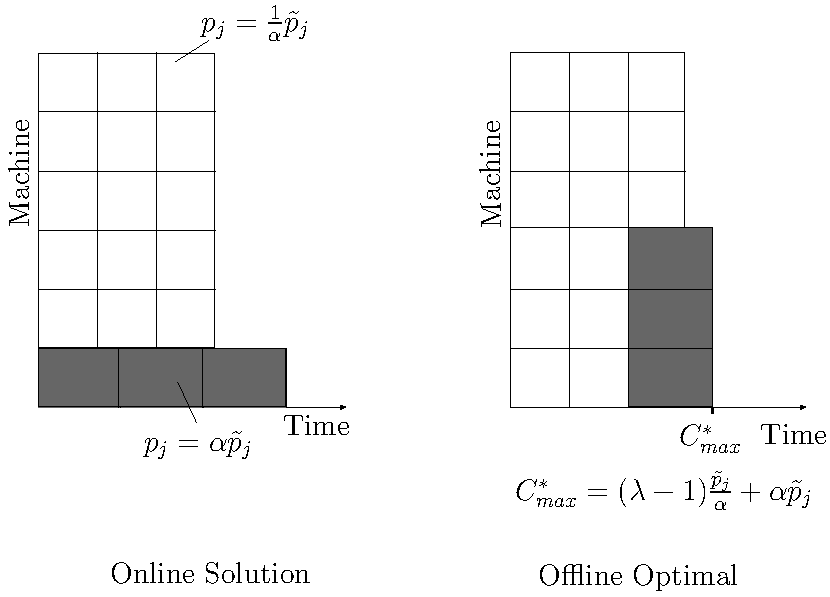
\includegraphics[width= 12 cm]{model1.pdf}
     \caption{Instance constructed by the adversary in the proof of
       theorem~\ref{th:model1-lb} with $\lambda = 3$ and $m = 6$. In the
       online solution, the adversary increases 
       the processing time of a task of the most loaded machine by a factor of $\alpha$. If
       that information was available beforehand, an optimal offline
       algorithm could have distributed these longer tasks to other
       processors.}
     \label{fig:rara}
     \end{figure}
   \end{myproof}    
     
     
     \begin{corollary}
     When $m$ goes to $\infty$ there is no online algorithm having competitive ratio better than $\alpha^{2}$.
     \end{corollary}
     
   \bodysubsection{Algorithm}
   
   We present the algorithm \textit{LPT-No Choice}. In phase 1, the
   algorithm distribute the data of the tasks to the processor using
   their estimated processing times according to Graham's LPT
   algorithm~\cite{Graham69boundson}: The tasks are sorted in non-increasing
   order of their processing time and are greedily scheduled on the
   processor that minimizes the sum of $\tilde{p_j}$ of the tasks
   allocated on that processor. Since there is no replication, there is
   no decision to take in phase 2.
   
   The performance of the algorithm depends mostly on how much the actual
   processing times of the tasks differ from their estimation. It also depends on the
   existence of a better arrangement if the actual processing times were
   known. The following theorem states the theoretical guarantee of the
   algorithm.
   
   \begin{theorem}
   \label{th:strat1-ub}
   The \textit{LPT-No Choice} has a competitive ratio of $ \frac{2\alpha^{2}m}{2\alpha^{2}+ m-1}$.
   \end{theorem} 
   
   \begin{myproof}
     The algorithm assigns the jobs to processors based on their
     estimated processing times using LPT in Phase 1. So, the
     planned makespan considering the estimated processing times of tasks,
     $\tilde{C}_{max}$ have the following relation with the total
     estimated processing time, $\tilde{p_j}$ and estimated processing
     time of the task  $l$ that reaches $\tilde{C}_{max}$.
   \begin{equation}\label{eq2}
   \tilde C_{max}\leq  \frac{\sum{\tilde p_j + (m-1) \tilde p_l} }{m}
   \end{equation}
   
   The actual makespan of a schedule, $C_{max}$, obtained using the
   actual processing times of all the jobs, must be smaller than $C_{max} \leq \alpha
   \tilde C_{max}$ (thanks to Equation~\ref{eq1}). We
   have following inequality:
   \begin{equation}\label{eq3}
     C_{max}\leq \alpha \tilde C_{max}\leq \alpha \left ( \frac{\sum{\tilde p_j + (m-1) \tilde p_l} }{m} \right )
   \end{equation} 
   
   The worst case situation is when the task of the processor where the
   sum of estimated processing time is $\tilde C_{max}$ sees the actual
   processing time of its task being $\alpha$ times larger than their
   estimate; meanwhile the processing time of the task on the rest of the
   processors is $\frac{1}{\alpha}$ times their estimation. The argument
   behind this statement is that greater the value of ratio
   $\frac{C_{max}}{\sum{p_j}}$, the worse the algorithm approximation
   ratio will be. So the total actual processing time is
   given by the following equation.
    \begin{equation}\label{eq4}
    \sum {p_j} = \frac{\sum \tilde{p_j}- \tilde{C_{max}}}{\alpha} + \alpha \tilde C_{max}
    \end{equation}
    
    Also the actual optimal makespan have following constraint
    \begin{equation}\nonumber 
   C_{max}^{*}\geq \frac{\sum {p_j}}{m}
   \end{equation}
   
   Substituting for  $ \sum {p_j}$, we have
    \begin{equation}\nonumber 
    m C_{max}^{*}\geq \frac{\sum \tilde{p_j}- \tilde{C_{max}}}{\alpha} + \alpha \tilde C_{max}
    \end{equation} 
   \begin{equation}\nonumber 
    m C_{max}^{*}\geq \frac{\sum \tilde{p_j} - \left( \frac{\sum{\tilde{p_j} + (m-1) \tilde{p_l} }}{m} \right )} {\alpha} + {C_{max}}
   \end{equation}
   \begin{equation}\nonumber
    m C_{max}^{*}\geq \frac{m-1}{\alpha m} \left( \sum \tilde p_j - \tilde{p_l} \right) + {C_{max}}
    \end{equation}
   
    By the property of LPT, $\sum \tilde p_j-\tilde p_l \geq m (\tilde C_{max}-\tilde p_l)$, we have,
   \begin{equation}\nonumber 
     m C_{max}^{*}\geq \frac{m-1}{\alpha } \left( \tilde{C_{max}} - \tilde{ p_l} \right) + {C_{max}}
    \end{equation}
    
    All instances where there is only one task per processor is always
    optimal. Therefore, we can restrict our analysis without loss of
    generality to instances with at least two jobs per processor. (Notice
    that in the original proof of Graham's LPT~\cite{Graham69boundson},
    an argument is made that all instances with two tasks per machine are
    optimal. However, the argument does not port in our case where only
    estimated processing times are known.) For at least two jobs on the
    processor that reaches $\tilde{C}_{max}$, the (estimated)
    processing time of last job is smaller than half the estimated
    makespan, $\tilde{p_l} \leq \frac{\tilde{C}_{max}}{2}$. Substituting
    this expression in the above equation, we have
   \begin{equation}\nonumber
    m C_{max}^{*}\geq \frac{m-1}{\alpha } \left( \tilde C_{max}-\frac{\tilde C_{max}}{2} \right ) + {C_{max}}
   \end{equation}
   
   Using equation~\ref{eq3},
   \begin{equation}\nonumber
    m C_{max}^{*}\geq \frac{m-1}{2\alpha } \frac{C_{max}} {\alpha} + {C_{max}}
   \end{equation}
   \begin{equation}\nonumber
    m C_{max}^{*}\geq \left( \frac{m-1}{2\alpha^{2} } +1\right){C_{max}}
   \end{equation}
   \begin{equation}\nonumber
   \frac{C_{max}}{C_{max}^{*}}\leq \frac{2\alpha^{2}m}{2\alpha^{2}+ m-1}
   \end{equation}
   \end{myproof} 
   
   \bodysection{Strategy 2: Replicate Data Everywhere}
   With this strategy, we put no restriction on phase 2. The tasks are
   replicated everywhere i.e. $\forall j, |M_{j}|=|M|$. We introduce the
   \textit{LPT-No Restriction} which replicates the data of all the tasks
   on each machine in the first phase. In the second phase we simply use
   the Longest Processing Time algorithm (LPT) in an online fashion using
   the estimated processing time of the task. That is to say, the tasks
   are sorted in non-increasing order of their estimated processing
   time. Then the task are greedily allocated on the first
   processor that becomes available. Note that this is done in phase 2,
   the processor become available with when the actual processing time of
   the task scheduled onto it elapse.
   
   \begin{lemma}\label{No Restriction}
     Let $l$ be the task that reaches $C_{max}$ in the solution
     constructed by \textit{LPT-No Restriction}. If there are at least two
     tasks on the machine that executes $l$ in \textit{LPT-No Restriction}, then 
     $C_{max}^* \geq {\frac{2}{\alpha^{2}}} p_l$.
   \end{lemma}
   \begin{myproof}
     Since there are at least two tasks on the machine that executes $l$
     in \textit{LPT-No Restriction}, there are at least $m+1$ tasks $i$
     such that $\tilde{p_j} \geq \tilde{p_l}$. Therefore in any solution
     at least one machine gets two tasks $c$ and $d$, such that $\tilde
     p_c \geq \tilde p_l$ and $\tilde p_d \geq \tilde p_l$. $C_{max}^{*}$
     must be greater than sum of the processing time of these two tasks.
      \begin{equation}\nonumber
       C_{max}^{*}\geq p_c + p_d
     \end{equation}	
   
     As the actual processing time of a task must be greater than  $\frac{1}{\alpha}$ times of its estimated value, we have $p_c \geq \frac{1}{\alpha}\tilde{p_c}$ and $p_d \geq \frac{1}{\alpha}\tilde{p_d}$. Using this
     \begin{equation}\nonumber 
       C_{max}^{*} \geq \frac{1}{\alpha}\tilde p_c +  \frac{1}{\alpha} \tilde p_d \geq \frac{2}{\alpha}\tilde p_l
     \end{equation}
   Since, $\tilde p_l \geq \frac{1}{\alpha} p_l$, we have
     \begin{equation}\nonumber
       C_{max}^{*} \geq {\frac{2}{\alpha^{2}}} p_l 
     \end{equation}
   \end{myproof}
   
   \begin{theorem}
     \label{th:strategy2}
     \textit{LPT-No Restriction} has a competitive ratio of
     $\frac{C_{max}}{C_{max}^{*}} \leq 1 + (\frac{m-1}{m})
     \frac{\alpha^{2}}{2}$
   \end{theorem} 
   
   \begin{myproof}
     The optimal makespan, $C_{max}^{*}$ must be at least equal to the
     average load on the $m$ machines. We have
     \begin{equation}\label{eq7}
       C_{max}^{*}\geq\frac{\sum p_j}{m}
     \end{equation}
   
     By the property of LPT (actually, it is a property of List
     Scheduling which LPT is a refinement of) the load on each machine
     $i$ is greater than the load on the machine which reach $C_{max}$
     before the last task $l$ is scheduled. So for each machine $i$,
     $C_{max} \leq \sum_{j \in E_i}^{}{p_j} + p_l$ holds true.  Summing
     for all the machines we have
     \begin{equation}\nonumber
       mC_{max} \leq  \sum {p_j} + (m-1)p_l
     \end{equation}
     \begin{equation}\label{eq8}
       C_{max} \leq  \frac{\sum {p_j}}{m} + \frac{(m-1)}{m}p_l
     \end{equation}
     
     Using~\ref{eq7} and~\ref{eq8}, we have
     \begin{equation}\nonumber
       \frac{C_{max}}{C_{max}^{*}} \leq 1 + {\frac{m-1}{m}}\left(\frac{p_l}{C_{max}^{*}}\right)
     \end{equation}
     
     Using Lemma~\ref{No Restriction}, we have 
     \begin{equation}\nonumber
       \frac{C_{max}}{C_{max}^{*}} \leq 1 + \left(\frac{m-1}{m}\right)\frac{\alpha^{2}}{2}
     \end{equation}
   
   \end{myproof}  
   
   Graham's List Scheduling algorithm always has a competitive ratio
   of $2-\frac{1}{m}$. For $\alpha^2 < 2$, the \textit{LPT-No
     Restriction} algorithm has better approximation than List
   Scheduling. For $\alpha^2 > 2$ List Scheduling has better guarantee
   than the one expressed in Theorem~\ref{th:strategy2}. Since
   \textit{LPT-No Restriction} is a variant of List Scheduling,
   the algorithm has a competitive ratio of $\min (1 +
   \frac{m-1}{2m}\alpha^{2}, 2-\frac{1}{m})$.
   \bodysection{Strategy 3: Replication in Groups}
   This strategy partitions the processors into $k$ groups
    $G1$,$G2$...$Gk$. The size of each group is equal and have
    $\frac{m}{k}$ processors within each group. For the sake of
    simplicity, we assume that we will only use values of $k$ such that
    $k$ divides $m$. In the first phase, the data of each task is
    replicated on all the processors of one of the $k$ groups,
    i.e. $\forall j, |M_j|= \frac{m}{k}$. In the second phase the tasks
    are scheduled within the group they are assigned to in first phase.
    Figure \ref{fig:Model 3} shows the construction of two phases.
    
    We propose the \textit{LS-Group} algorithm which is based on Graham's
    List Scheduling algorithm. In phase 1, we use List Scheduling to
    distribute the tasks to the $k$ groups of processors. In phase 2 each
    task is scheduled to a particular processor within the group it was
    allocated in phase 1 using the online List Scheduling algorithm.
    
    \begin{figure*}[htp] 
    \centering
    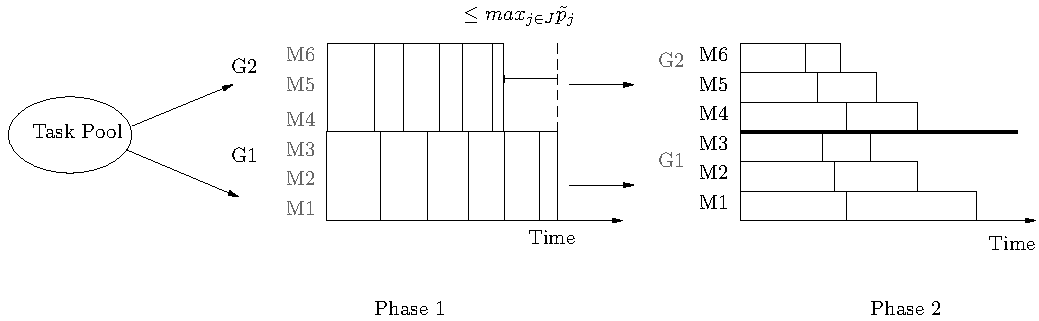
\includegraphics[width=\linewidth]{model3.pdf}
    \caption{An example of replication in groups with $m = 6$, $k = 2$. In
      phase 1, the data of the tasks are assigned to one of the
      groups. Phase 2 schedules each task assigned to a machine within its
      group.}
    \label{fig:Model 3}
    \end{figure*}
    
    \begin{theorem}
      \label{th:strategy3}
      With $k$ groups, the competitive ratio of
      \textit{LS-Group } is $ \frac{k\alpha^{2}}{\alpha^{2}+k-1} (1+
      {\frac{k-1}{m}} ) + \frac{m-k}{m}$
    \end{theorem}
    \begin{myproof} 
      We assume without loss of generality that $ C_{max}$ comes from
      group $G1$. $C_{max}^{*}$ must be greater than the average of the
      loads on the machines.
      \begin{equation}{\nonumber}
        C_{max}^{*} \geq  \frac{\sum_{j \in J}^{}{{p_{j}}}}{m}
      \end{equation}
    
      $\sum_{j \in J }{{p_{j}}}$ can be written as sum of load on $G1$ and
      load on rest of groups.
      \begin{equation}\label{eq11}
        C_{max}^{*} \geq  \frac{\sum_{j \in G1 }^{}{{p_{j}}}+ \sum_{l=2}^{k}\sum_{j \in Gl }^{}{{p_{j}}}}{m}
      \end{equation}
    
      As in phase 1 tasks are allocated to different groups using List
      Scheduling with the estimated processing times of the tasks, the
      (estimated) load difference between any two groups cannot be greater
      than the estimated value of largest task ${max_{j \in J}}{\tilde
        p_{j}}$.  So, for any group $Gl \neq G1$, We have
      \begin{equation}{\nonumber}
    \forall l \in \{2, 3, \dots ,k\}, |\sum_{j \in G1 }^{}{\tilde p_{j}}- \sum_{j \in Gl }^{}{\tilde p_{j}}| \leq {max_{j \in J}}{\tilde p_{j}}
      \end{equation}  
      Adding for all values of $l$ leads to
      \begin{equation}{\nonumber}
        |(k-1)\sum_{j \in G1 }^{}{\tilde p_{j}}- \sum_{l=2}^{k}\sum_{j \in Gl }^{}{\tilde p_{j}}| \leq (k-1) {max_{j \in J}}{\tilde p_{j}}
      \end{equation}
    
      \textit{Case 1:} If $(k-1)\sum_{j \in G1 }^{}{\tilde p_{j}} >
      \sum_{l=2}^{k}\sum_{j \in Gl }^{}{\tilde p_{j}}$.
      \begin{equation}{\nonumber}
        \sum_{l=2}^{k}\sum_{j \in Gl }^{}{\tilde p_{j}} \geq (k-1) \left( \sum_{j \in G1 }^{}{\tilde p_{j}}- {max_{j \in J}}{\tilde p_{j}} \right)
      \end{equation}
    
      As the actual processing time of the tasks can vary within a factor
      $\alpha$ and $\frac{1}{\alpha}$ of their estimated processing time,
      the following inequality holds
      \begin{equation}{\nonumber}
        \alpha\sum_{l=2}^{k}\sum_{j \in Gl }^{}{{p_{j}}} \geq (k-1) \left( \frac{1}{\alpha}\sum_{j \in G1 }^{}{{p_{j}}}- \alpha {max_{j \in J}}{{p_{j}}} \right)
      \end{equation}
      \begin{equation}\label{eq9}
        \sum_{l=2}^{k}\sum_{j \in Gl }^{}{{p_{j}}} \geq (k-1) \left(\frac{1}{\alpha^{2}}\sum_{j \in G1 }^{}{{p_{j}}}-  {max_{j \in J}}{{p_{j}}} \right)
      \end{equation}
    
      Phase 2 applies List Scheduling in the online mode. We assumed that
      $C_{max}$ comes from $G1$. Using the guarantees of List Scheduling
      we can write,
      \begin{equation}\label{eq10}
        C_{max} \leq \frac{\sum_{j \in G1 }^{}{{p_{j}}}}{m/k} + {\frac{m/k-1}{m/k}} p_{max}
      \end{equation}
      where $p_{max}$ is actual processing time of longest task in $G1$.
    
      From Equation~\ref{eq9} and~\ref{eq11}, we derive
      \begin{equation}{\nonumber}
        C_{max}^{*} \geq  \frac{\sum_{j \in G1 }^{}{{p_{j}}}+ (k-1)\left(\frac{1}{\alpha^{2}}\sum_{j \in G1 }^{}{{p_{j}}}-  {max_{j \in J}}{{p_{j}}}\right)}{m}
      \end{equation}
      \begin{equation}{\nonumber}
        \alpha^{2} (mC_{max}^{*} + (k-1){max_{j \in J}}{{p_{j}}}) \geq  (\alpha^{2} + k-1) \sum_{j \in G1 }^{}{{p_{j}}}  
      \end{equation}
      \begin{equation}\label{eq12}
        \frac{\alpha^{2}}{\alpha^{2}+k-1}\left(m C_{max}^{*}+(k-1) {max_{j \in J}}{{p_{j}}}\right) \geq \sum_{j \in G1 }^{}{{p_{j}}}  
      \end{equation}
      
      Using \ref{eq10} and \ref{eq12}, We have
      \begin{align}{\nonumber}
        C_{max} \leq \frac{k\alpha^{2}}{\alpha^{2}+k-1}\left( C_{max}^{*}+\frac{k-1}{m} {max_{j \in J}}{{p_{j}}}\right)\\
        + {\frac{m/k-1}{m/k}} p_{max} \nonumber
      \end{align}
      
      As $C_{max}^{*}\geq {{max_{j \in J}}{p_{j}}}\geq p_{max}$, we have
      \begin{align}{\nonumber}
        C_{max} \leq \frac{k\alpha^{2}}{\alpha^{2}+k-1}\left( C_{max}^{*}+ {\frac{k-1}{m}}{C_{max}^{*}}\right)\\
        + {\frac{m-k}{m}} C_{max}^{*} \nonumber
      \end{align}    
      
      So, in Case 1 the algorithm has a competitive ratio of,
      \begin{equation}{\nonumber}
        \frac{C_{max}}{C_{max}^{*}} \leq \frac{k\alpha^{2}}{\alpha^{2}+k-1}\left( 1+ {\frac{k-1}{m}} \right) + {\frac{m-k}{m}} \end{equation}\\
      
      \textit{Case 2:} If $(k-1)\sum_{j \in G1 }^{}{\tilde p_{j}} \leq \sum_{l=2}^{k}\sum_{j \in Gl }^{}{\tilde p_{j}}$. \\
      
      Since the processing times of the tasks can vary within a factor
      $\alpha$ and $\frac{1}{\alpha}$ of their estimated values, the
      expression for case 2 can be written as
      \begin{equation}{\nonumber}
        \sum_{l=2}^{k}\sum_{j \in Gl }^{}{ p_{j}} \geq \frac{1}{\alpha^2} (k-1)\sum_{j \in G1 }^{}{ p_{j}}
      \end{equation}
      
      Putting this value in Equation~\ref{eq11}, we have
      \begin{equation}\label{eq13}
        C_{max}^{*} \geq \frac{\alpha^2+k-1}{m\alpha^2}\sum_{j \in G1 }^{}{ p_{j}}
      \end{equation}
      Using Equations~\ref{eq10} and~\ref{eq13}, and as $C_{max}^{*} \geq p_{max}$, we have
      \begin{equation}{\nonumber}
        C_{max} \leq \frac{k\alpha^2}{\alpha^2+k-1}C_{max}^{*}+\frac{m-k}{m}C_{max}^{*}
      \end{equation}
      
      So, in case 2 the algorithm has a competitive ratio of
      $\frac{k\alpha^2}{\alpha^2+k-1}+\frac{m-k}{m}$.
    
      Clearly, the algorithm has a worst competitive ratio in case 1.  So,
      the algorithm has a competitive approximation ratio of
      $\frac{C_{max}}{C_{max}^{*}} \leq \frac{k\alpha^{2}}{\alpha^{2}+k-1}
      \left( 1+ {\frac{k-1}{m}} \right) + {\frac{m-k}{m}}$.
    \end{myproof}
    
    % \begin{corollary}
    %   When there are $2$  groups, the competitive ratio is $ 1+
    %   \frac{2}{1+\alpha^{2}} (\alpha^2-\frac{1}{m})$.
    % \end{corollary}
    
    \textit{LS-Group} uses List Scheduling in both its phases. A LPT-based
    algorithm may have better guarantee. But without performing any
    replication, {\em i.e.} when $k=m$, the \textit{LS-Group} algorithm
    has a competitive ratio almost equal to \textit{LPT-No choice}'s when
    the number of machines $m$ is large and the value of $\alpha$ is
    within practical range. This indicates an LPT-based algorithm for
    strategy 3 would likely not have a much more interesting guarantee.
    \bodysection{Summary}\label{ch4:summary}
     Table~\ref{tab:template} summarizes the results of this chapter in term
     of approximation theory. Based on adversary technique,
     Theorem~\ref{th:model1-lb} states that there is no algorithm which can
     give performance better than $\frac{\alpha^{2}m }{\alpha^{2} + m-1}$ for the model where no
     replication is allowed. {\it LPT-No Choice} is a
     $\frac{2\alpha^{2}m}{2\alpha^{2}+ m-1}$-approximation that uses that
     strategy. For the second strategy that replicates the data of all
     tasks everywhere ( $|M_j| = |M|$), {\it LPT-No Restriction} achieves a
     competitive ratio of $1 + (\frac{m-1}{m})\frac{\alpha^{2}}{2}$.  The
     third strategy uses replication within $k$ groups of size $m/k$ ({\em
       i.e.}, $|M_j| = m/k$). Using this strategy, the {\it LS-Group}
     algorithm has a competitive ratio of
     $\frac{k\alpha^{2}}{\alpha^{2}+k-1}\left( 1+ {\frac{k-1}{m}} \right) +
     {\frac{m-k}{m}}$.\\
     
     
     
     \begin{table}[ht]
       \centering
       \begin{tabular}{|l|c|c|c|c|c|}
         \hline
         Replication & Approximation ratio  \\
         \hline
         $|M_j|=1$ & $\frac{C_{max}}{C_{max}^{*}}\leq \frac{2\alpha^{2}m}{2\alpha^{2}+ m-1}$ (Th.~\ref{th:strat1-ub})  \\
         & No approximation better than $\frac{\alpha^{2}m }{\alpha^{2} + m-1}$ (Th.~\ref{th:model1-lb})   \\
         
         \hline
         $|M_j|=m$ & $\frac{C_{max}}{C_{max}^{*}} \leq 1 + (\frac{m-1}{m})\frac{\alpha^{2}}{2}$ (Th.~\ref{th:strategy2})  \\
         & $\frac{C_{max}}{C_{max}^{*}} \leq 2-\frac{1}{m}$ \cite{Graham66}   \\
         \hline
         
         $|M_j|= \frac{m}{k} $ & $\frac{C_{max}}{C_{max}^{*}} \leq \frac{k\alpha^{2}}{\alpha^{2}+k-1} \left(1+ {\frac{k-1}{m}} \right)+ {\frac{m-k}{m}}$ (Th.~\ref{th:strategy3})  \\
     %    & $\frac{C_{max}}{C_{max}^{*}} \leq  1+ \frac{2}{1+\alpha^{2}} \left(\alpha^2-\frac{1}{m}\right)$ when $k=2$ [Col. 3.1]   \\
         
         \hline
       \end{tabular}
       \caption{Summary of the contribution of this chapter.
         Three proposed algorithms have guaranteed performance.
         One lower bound on approximability has been established.}
       \label{tab:template}
     \end{table}
     
     
     Of course, there is an inherent tradeoff between replicating data and   obtaining good values for the makespan. To better understand the   tradeoff we show in Figure~\ref{fig:Graph} how the expressions of the   guarantees (or impossibility)translate to actual values in a  approximation ratio / replication space.  We picked 3 values of   $\alpha$ while keeping the number of machines fixed $m=210$. 
     
     When $\alpha=1.1$, even with multiple groups {\it LS-Group} provides little improvement over {\it LPT-No Choice}. However there is a significant  gap between the guarantee of {\it LPT-No Choice} and the lower bound  on possible approximation. When $\alpha$ is small, there is a  significant improvement in using {\it LPT-No Restriction} over using  simply {\it LS-Group} with only 1 group.
     
     When $\alpha$ increases to $1.5$, there is no more differences in the  guarantees of {\it LS-Group} with 1 group and {\it LPT-No
       Restriction}. Also {\it LS-Group} provides many intermediate  solution between deploying the data on a single machine and deploying
     them everywhere.
     
     When $\alpha=2$, the range of the approximation ratios increase and
     the value of the lower bound increases. Now {\it LS-Group} is able to
     get a better approximation using less than $50$ replications than is
     possible by deploying data on a single machine. Also, the
     approximation ratio quickly improves from more than $7.5$ with the
     data being replicated on $1$ machine to a ratio of less than $6$ with
     only replicating the data on $3$ machines.
     
     Overall, when $\alpha$ is large, only few replication improve the
     performance significantly.
     
     
     \begin {figure}
       \centering
       \begin{subfigure}[b]{0.5\textwidth}
         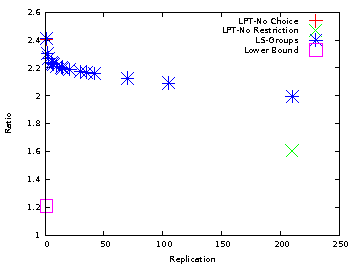
\includegraphics[width=\textwidth]{alpha_11.pdf}
         \caption{$m=210$, $\alpha=1.1$}
         \label{fig:1}
       \end {subfigure} %
       
       \begin{subfigure}[b]{0.5\textwidth}
         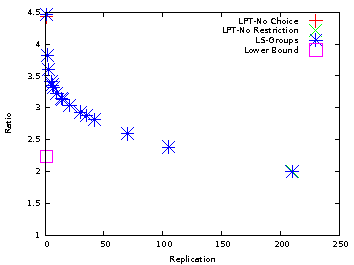
\includegraphics[width=\textwidth]{alpha_15.pdf}
         \caption{$m=210$, $\alpha=1.5$}
         \label{fig:2}
       \end {subfigure} %
       
       \begin{subfigure}[b]{0.5\textwidth}
         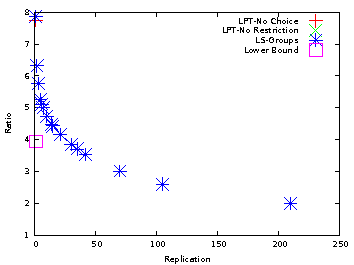
\includegraphics[width=\textwidth]{alpha_2.pdf}
         \caption{$m=210$, $\alpha=2$}
         \label{fig:3}
       \end{subfigure} %
     
       \caption{Ratio-Replication graph with $m=210$ and $\alpha \in \{1.1, 1.5, 2\}$.}
       \label{fig:Graph}
     \end{figure}
   
   \bodychapter{MEMORY AWARE REPLICATION UNDER UNCERTAINTY}\label{ch5}
   
   
    Replication improves performance but incurs a cost in terms of memory consumption.  
    Replication allows to obtain a better load balancing by reducing the effect of 
    uncertainties in processing times of tasks. But each replica occupies memory, and increases the memory consumption. 
    So, replicating all the tasks is not possible in real scenarios. This justify the need for an efficient replication 
    strategy which allows an algorithm to choose which tasks are to be replicated and where.
    In this chapter we investigate the bi-objective problem of minimizing the makespan as well as the memory consumption. A memory-aware replication strategy improves execution times with little increase in memory consumption. 
    \bodysection{Preliminaries}
   
    The problem is to schedule a set $J$ of $n$ tasks on $m$ machines such that both makespan $C_{max}$ as well as memory usage $M_{max}$ is optimized.  
     Let $\pi_1$ be the schedule  which minimizes makespan and $\pi_2$ be the memory-aware schedule. $\tilde{C}^{\pi_1}_{max}$ and $\tilde{C}^{*}_{max}$ are makespan and optimal makespan when all the tasks are scheduled according to $\pi_1$. Similarly, $M^{\pi_2}_{max}$ is  memory consumption of the most  occupied machine and $M^*_{max}$ is its optimal value. The strategy is to divide tasks into two sets $S_1$ and $S_2$ such that set $S_1$ contains the processing time intensive tasks and set $S_2$ contains the memory intensive tasks, and schedule them differently and in such a way that it optimizes both the objectives. 
     
     We propose two algorithms $SABO_\triangle$ (stands for static asymmetric bi-objective) and $ABO_\triangle$ (stands for asymmetric bi-objective), which are based on $SBO_\triangle$ algorithm. $SBO_\triangle$~\cite{10.1109/IPDPS.2008.4536292} is bi-objective algorithm for minimizing makespan and memory usage for independent tasks by combining results of two symmetric schedules each dedicated to a single objective.
     
      \bodysection{The $SABO_\triangle$ Algorithm}
                     
                     We propose $SABO_\triangle$ Algorithm which is static in nature and restrict each task to be scheduled to only one machine. Similar to $SBO_\triangle$ this algorithm assigns tasks to all the machines in phase 1 such that it minimizes both the objectives. As each task is restricted to only one machine, there is no task replication. Based on similar condition as in $SBO_\triangle$, a processing-time intensive task is assigned to $\pi_1$ schedule and a memory intensive task is assigned to $\pi_2$
                     
                     In phase 2, the algorithm loads the tasks to the machines they were assigned in phase 1.\\
                     
                       \begin{figure}[htp]
                       \centering
                       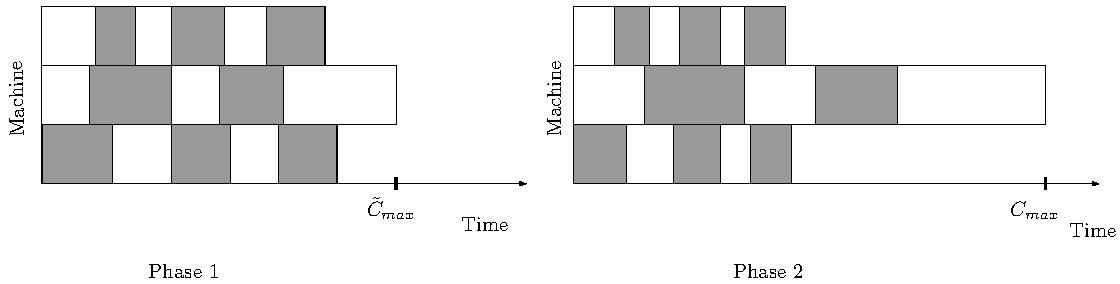
\includegraphics[width= 16 cm]{mem2.pdf}
                       \caption{An example of two phases of the schedule generated by the $SABO_\triangle$. The uncolored parts  represent tasks scheduled according $\pi_2$. The colored parts represents tasks scheduled according $\pi_1$}
                       \label{fig:ch5-1}
                       \end{figure} 
                         \begin{algorithm}                    
                         \caption{$SABO_\triangle$}
                         \label{alg2}
                          \begin{algorithmic} 
                          \State \textbf{Input:} $m$ machines 
                          \State \hspace*{42pt}Set $J$ of $n$ tasks
                          \State\hspace*{42pt}Let $\pi_1$ be a $ \rho_1$-approximated schedule on makespan $\tilde{C}_{max}$ 
                         \State \hspace*{42pt}Let $\pi_2$ be a $\rho_2$- approximated schedule on memory ${M_{max}}$
                         \State
                          \State \textbf{Phase 1:} [Uses $SBO_\triangle$]
                       \ForAll{$j\in J$}
                       \If{$\frac{\tilde{p_j}}{\tilde{C}^{\pi_1}_{max}} \leq \triangle \frac{s_j}{M^{\pi_2}_{max}}$}
                       \State Assign $j$ to a machine according to $\pi_2$ schedule
                       \State Add $j$ to $S_2$
                       \Else
                       \State Assign $j$ to a machine according to $\pi_1$ schedule
                       \State Add $j$ to $S_1$   
                       \EndIf 
                       \EndFor
                      
                        \State \textbf{End of Phase 1} 
                        \State 
                         \State \textbf{Phase 2:} 
                         \State \hspace*{42pt}Schedule tasks to machines to which they were assigned during phase 1
                            
                         \State \textbf{End of Phase 2} 
                          
                               \end{algorithmic}
                               \end{algorithm}     
           
                             
                            
                            \begin{theorem}
                            \label{th:chapter5-2a}
                             The $SABO_\triangle$ Algorithm generates a $(1+\triangle)\alpha^2 \rho_1$ - approximated schedule on makespan.
                            \end{theorem}         
                            \begin{myproof}
                            Let $k$ be the machine reaching the makespan $C_{max}$ of the schedule. $C_{max}$ can be written as the sum of processing times of tasks in set $S_1$ and $S_2$ scheduled on machine $k$.
                            \begin{equation}\nonumber
                      C_{max}= \sum_{j \in S_1 \cap E_k}^{}p_j+\sum_{j \in S_2 \cap E_k}^{}p_j 
                            \end{equation}
                            
                            Since, $\sum\limits
                            _{j \in S_2 \cap E_k}^{}p_j\leq\alpha\sum\limits
                            _{j \in S_2 \cap E_k} \tilde{p}_j$
                              \begin{equation}\nonumber
                              C_{max} \leq \sum_{j \in S_1 \cap E_k}^{}p_j+\alpha\sum_{j \in S_2 \cap E_k} \tilde{p}_j 
                                    \end{equation}
                           
                            
                            Let $C^{\pi_1}_{max}$ denotes the makespan obtained after phase 2 when tasks are loaded and actual processing time of a task is known to scheduler. Since $C^{\pi_1}_{max} \geq \sum\limits
                            _{j \in S_1 \cap E_k}^{}p_j$ and $\sum\limits
                            _{j \in S_2\cap E_k}\triangle {\tilde{C}^{\pi_1}_{max}} \frac{s_j}{M^{\pi_2}_{max}}\geq \sum\limits
                            _{j \in S_2\cap E_k}^{}\tilde{p}_j $ by definition of $S_2$, we have
            \begin{equation}\nonumber
        C_{max}\leq C^{\pi_1}_{max}+\alpha\sum_{j \in S_2\cap E_k}^{}\triangle {\tilde{C}^{\pi_1}_{max}} \frac{s_j}{M^{\pi_2}_{max}}
                                   \end{equation}                    
          Since, $C^{\pi_1}_{max}\leq\alpha\tilde{C}^{\pi_1}_{max}$ and $\sum\limits_{j \in S_2\cap E_k} \frac{s_j}{M^{\pi_2}_{max}}\leq 1$, we have
            \begin{equation}\nonumber                       C_{max}\leq(1+\triangle)\alpha\tilde{C}^{\pi_1}_{max}                         \end{equation}
         
        Since $ \tilde{C}^{\pi_1}_{max} \leq \rho_1 \tilde{C}^{*}_{max}\leq \alpha\rho_1 {C}^{*}_{max}$ the algorithm has an approximation ratio of $(1+\triangle)\alpha^2 \rho_1$ on makespan.
                                \end{myproof}
      \begin{theorem} \label{th:chapter5-2b}
        The $SABO_\triangle$ Algorithm generates $ (1+\frac{1}{\triangle})\rho_2 $- approximated schedule on memory 
         \end{theorem}                      
         \begin{myproof}  
         The proof is identical to $SBO_\triangle$ algorithm and is presented in chapter~\ref{ch3}.                                           
         \end{myproof}    
    
    \bodysection{The $ABO_\triangle$ Algorithm} 
    We propose a two phase algorithm. In phase 1 the algorithm assigns tasks to all the machines such that it minimizes both the makespan as well as memory consumption. The tasks having more memory value  in comparison to its processing time are scheduled using memory intensive schedule which aim at minimizing memory.  Similarly tasks which incur more processing time cost compared to memory cost are assigned to machines according to the makespan intensive schedule. These   tasks are replicated to all machines in order to provide better load balancing and hence minimized makespan. The algorithm in its phase 1 assigns all the memory intensive tasks to machines first, then chooses tasks having more processing time values compared to memory they consume.
    
    In phase 2, the algorithm loads the memory intensive  tasks to the machines they were assigned in phase 1 respecting the tasks assignment during phase 1. The algorithm schedule the time intensive tasks (replicated tasks) using Graham's List Scheduling after all the memory intensive tasks are scheduled. Figure~\ref{fig:ch5-2} shows a schedule instance using the algorithm.\\
    
      \begin{figure}[htp]
      \centering
      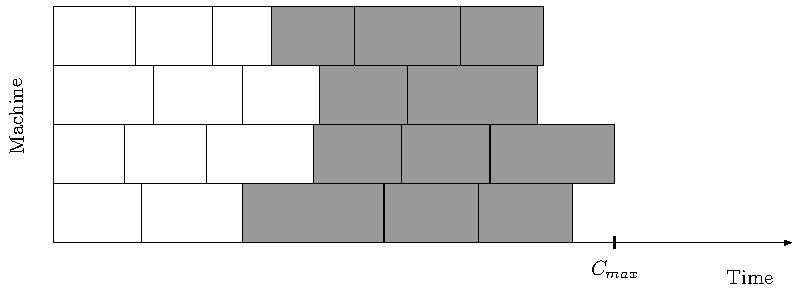
\includegraphics[width= 16 cm]{mem.pdf}
      \caption{An example of the schedule generated by the $ABO_\triangle$ algorithm. The uncolored parts represent the memory intensive tasks scheduled according $\pi_2$. The colored parts represent the processing time intensive tasks and scheduled using LS after replicated}
      \label{fig:ch5-2}
      \end{figure}
     \begin{algorithm}
     
     \caption{$ABO_\triangle$}
     \label{alg1}
      \begin{algorithmic} 
      \State \textbf{Input:} $m$ machines 
      \State \hspace*{42pt}Set $J$ of $n$ tasks
      \State\hspace*{42pt}Let $\pi_1$ be a $ \rho_1$-approximated schedule on makespan $\tilde{C}_{max}$ 
     \State \hspace*{42pt}Let $\pi_2$ be a $\rho_2$- approximated schedule on memory ${M_{max}}$
     \State
      \State \textbf{Phase 1:}
   \ForAll{$j\in J$}
   \If{$\frac{\tilde{p_j}}{\tilde{C}^{\pi_1}_{max}} \leq \triangle \frac{s_j}{M^{\pi_2}_{max}}$}
   \State Assign $j$ to a machine according to $\pi_2$ schedule
   \State Add task $j$ to set $S_2$   
   \EndIf 
   \EndFor
   \ForAll{$j\in J$}
   \If{$\frac{\tilde{p_j}}{\tilde{C}^{\pi_1}_{max}} \geq \triangle \frac{s_j}{M^{\pi_2}_{max}}$}
   \State Add $j$ to set $S_1$
   \State Replicate $j$ everywhere   
   \EndIf 
   \EndFor
    \State \textbf{End of Phase 1} 
    \State 
     \State \textbf{Phase 2:} 
     \State \hspace*{42pt}Schedule tasks from set $S_2$ respecting job assignment during phase 1
        \State \hspace*{42pt} Schedule all replicated tasks from set $S_1$ using Graham's LS Algorithm 
     \State \textbf{End of Phase 2} 
      
           \end{algorithmic}
           \end{algorithm}
         
           \begin{theorem}
           \label{th:chapter5-la}
            The $ABO_\triangle$ Algorithm  generates a $ (2-\frac{1}{m}+\triangle\alpha^2 \rho_1) $- approximated schedule on makespan.
           \end{theorem}         
           \begin{myproof}
           Let $k$ be the machine reaching the makespan $C_{max}$ of the schedule. $C_{max}$ can be written as the sum of the processing times of tasks in sets $S_1$ and $S_2$ scheduled on machine $k$.
           \begin{equation}\nonumber
     C_{max}= \sum_{j \in S_1 \cap E_k}^{}p_j+\sum_{j \in S_2 \cap E_k}^{}p_j 
           \end{equation}
           
           Since, $\sum\limits
           _{j \in S_2 \cap E_k}^{}p_j\leq\alpha\sum\limits
           _{j \in S_2 \cap E_k} \tilde{p}_j$
             \begin{equation}\nonumber
             C_{max} \leq \sum_{j \in S_1 \cap E_k}^{}p_j+\alpha\sum_{j \in S_2 \cap E_k} \tilde{p}_j 
                   \end{equation}
          
           
           Let $C^R_{max}$ denotes makespan obtained by scheduling the replicated tasks using LS. Since $C^R_{max} \geq \sum\limits
           _{j \in S_1 \cap E_k}^{}p_j$ and $\sum\limits
           _{j \in S_2\cap E_k}\triangle {\tilde{C}^{\pi_1}_{max}} \frac{s_j}{M^{\pi_2}_{max}}\geq \sum\limits
           _{j \in S_2\cap E_k}^{}\tilde{p}_j $ by definition of $S_2$, we have
           \begin{equation}\nonumber
            C_{max}\leq C^R_{max}+\alpha\sum_{j \in S_2\cap E_k}^{}\triangle {\tilde{C}^{\pi_1}_{max}} \frac{s_j}{M^{\pi_2}_{max}}
                  \end{equation}
            Using the property of LS, the approximation ratio of the schedule incorporating only replicated tasks is $2-\frac{1}{m}$. So, $C^R_{max} \leq (2-\frac{1}{m})C^{*}_{max}$. Also, $\sum\limits
            _{j\in S_2\cap E_k}^{} \frac{s_j}{M^{\pi_2}_{max}}\leq 1$. 
            \begin{equation}\nonumber
                    C_{max}\leq (2-\frac{1}{m})C^{*}_{max}+\alpha\triangle {\tilde{C}^{\pi_1}_{max}} 
                          \end{equation}
               Also,  ${\tilde{C}^{\pi_1}_{max}} \leq \rho_1 {\tilde{C}^{*}_{max}}$. Since $\tilde{C}^{*}_{max}$ is the optimal makespan obtained after phase 1 considering estimated processing times of the tasks, we have, $\tilde{C}^{*}_{max}\leq \alpha{C}^{*}_{max}$. So, ${\tilde{C}^{\pi_1}_{max}} \leq \alpha \rho_1{C}^{*}_{max}$. Using this, we have         
              \begin{equation}\nonumber
                            C_{max}\leq (2-\frac{1}{m}){{C}^{*}_{max}}+\alpha^2\triangle \rho_1 {{C}^{*}_{max}} 
                                  \end{equation}
               Hence, we proved that the algorithm generates a $(2-\frac{1}{m}+\triangle \alpha^2\rho_1) $- approximated schedule on makespan.
               \end{myproof}
               \begin{theorem}
                      \label{th:chapter5-lb}
                       The $ABO_\triangle$ Algorithm generates a $ (1+\frac{m}{\triangle})\rho_2 $- approximated schedule on memory.
                      \end{theorem}
        
             \begin{myproof}           
             When a task is replicated all its replica occupies space in memory and increase memory consumption. For $m$ replicas the total memory consumption is $m$ times of the replicated tasks. Similar to proof of previous theorem, the highest maximum memory occupied by any machine $k$ can be written as
              \begin{equation}\nonumber
              M_{max}= \sum_{j \in S_1\cap E_k}^{}s_j+\sum_{j \in S_2\cap E_k}^{}s_j           
           \end{equation}
           As each task in set $S_1$ is replicated over all the machines,$\sum\limits
           _{j \in S_1\cap E_k}^{}s_j =\sum\limits
           _{j \in S_1}^{}s_j$.              
               \begin{equation}\nonumber
                          M_{max} = \sum_{j\in S_1}^{}s_j+\sum_{j \in S_2\cap E_k}^{}s_j           
                       \end{equation}    
                        $\sum\limits_{j \in S_2\cap E_k}^{}s_j$  at most be equal to $M^{\pi_2}_{max} $ and $\sum\limits_{j\in S_1}s_j$ is bounded by $\sum\limits_{j \in J}^{} {M^{\pi_2}_{max}} \frac{\tilde{p_j}}{\triangle \tilde{C}^{\pi_1}_{max}} $ as per condition for  $\pi_1$ scheduling, using this we have    
    \begin{equation}\nonumber
    M_{max}\leq \sum_{j \in J}^{} {M^{\pi_2}_{max}} \frac{\tilde{p_j}}{\triangle \tilde{C}^{\pi_1}_{max}}+{M^{\pi_2}_{max}}
     \end{equation}
             Since $ \sum\limits_{j \in J}\tilde{p}_j \leq m\tilde{C}^{\pi_1}_{max} $, we have 
                 \begin{equation}\nonumber
     M_{max}\leq   \frac{m}{\triangle}{M^{\pi_2}_{max}}+{M^{\pi_2}_{max}}
   \end{equation}
    Also,  ${M^{\pi_2}_{max}} \leq \rho_2 {M^{*}_{max}}$.  Hence, The Algorithm generate $ (1+\frac{m}{\triangle})\rho_2 $- approximated schedule on memory.
                  \end{myproof}
                  
                  
    \bodysection{Summary}
     Table~\ref{tab:template2} summarizes the results for $SABO_\triangle$ and $ABO_\triangle$ algorithms. $SABO_\triangle$ is  similar to $ SBO_\triangle$ algorithm in its first phase and has a  approximation ratio of $[(1+\triangle)\alpha^2 \rho_1, (1+\frac{1}{\triangle})\rho_2]$ on makespan and memory.   $ABO_\triangle$ is a $ [(2-\frac{1}{m}+\triangle\alpha^2 \rho_1), (1+\frac{m}{\triangle})\rho_2] $-approximated algorithm on makespan and memory and replicate processing time intensive tasks to improve makespan.\\
     \\
     
     \begin{table}[ht]
         \centering
         \begin{tabular}{|l|c|c|c|c|c|}
           \hline
           Algorithm & Approx. on makespan & Approx. on memory  \\
           \hline
           $SABO_\triangle$&
           $(1+\triangle)\alpha^2 \rho_1$ (Th.~\ref{th:chapter5-2a})& $(1+\frac{1}{\triangle})\rho_2$ (Th.~\ref{th:chapter5-2b})   \\
           \hline
                   $ABO_\triangle$&
                   $(2-\frac{1}{m}+\triangle\alpha^2 \rho_1)$ (Th.~\ref{th:chapter5-la})& $(1+\frac{m}{\triangle})\rho_2$ (Th.~\ref{th:chapter5-lb})   \\
           
           
           
       %    & $\frac{C_{max}}{C_{max}^{*}} \leq  1+ \frac{2}{1+\alpha^{2}} \left(\alpha^2-\frac{1}{m}\right)$ when $k=2$ [Col. 3.1]   \\
           
           \hline
         \end{tabular}
         \caption{Summary of the results of the algorithm $SABO_\triangle$ and the algorithm $ABO_\triangle$.}
         \label{tab:template2}
       \end{table}
     
     
      \begin {figure*}
         \centering
         \begin{subfigure}[b]{0.5\textwidth}
           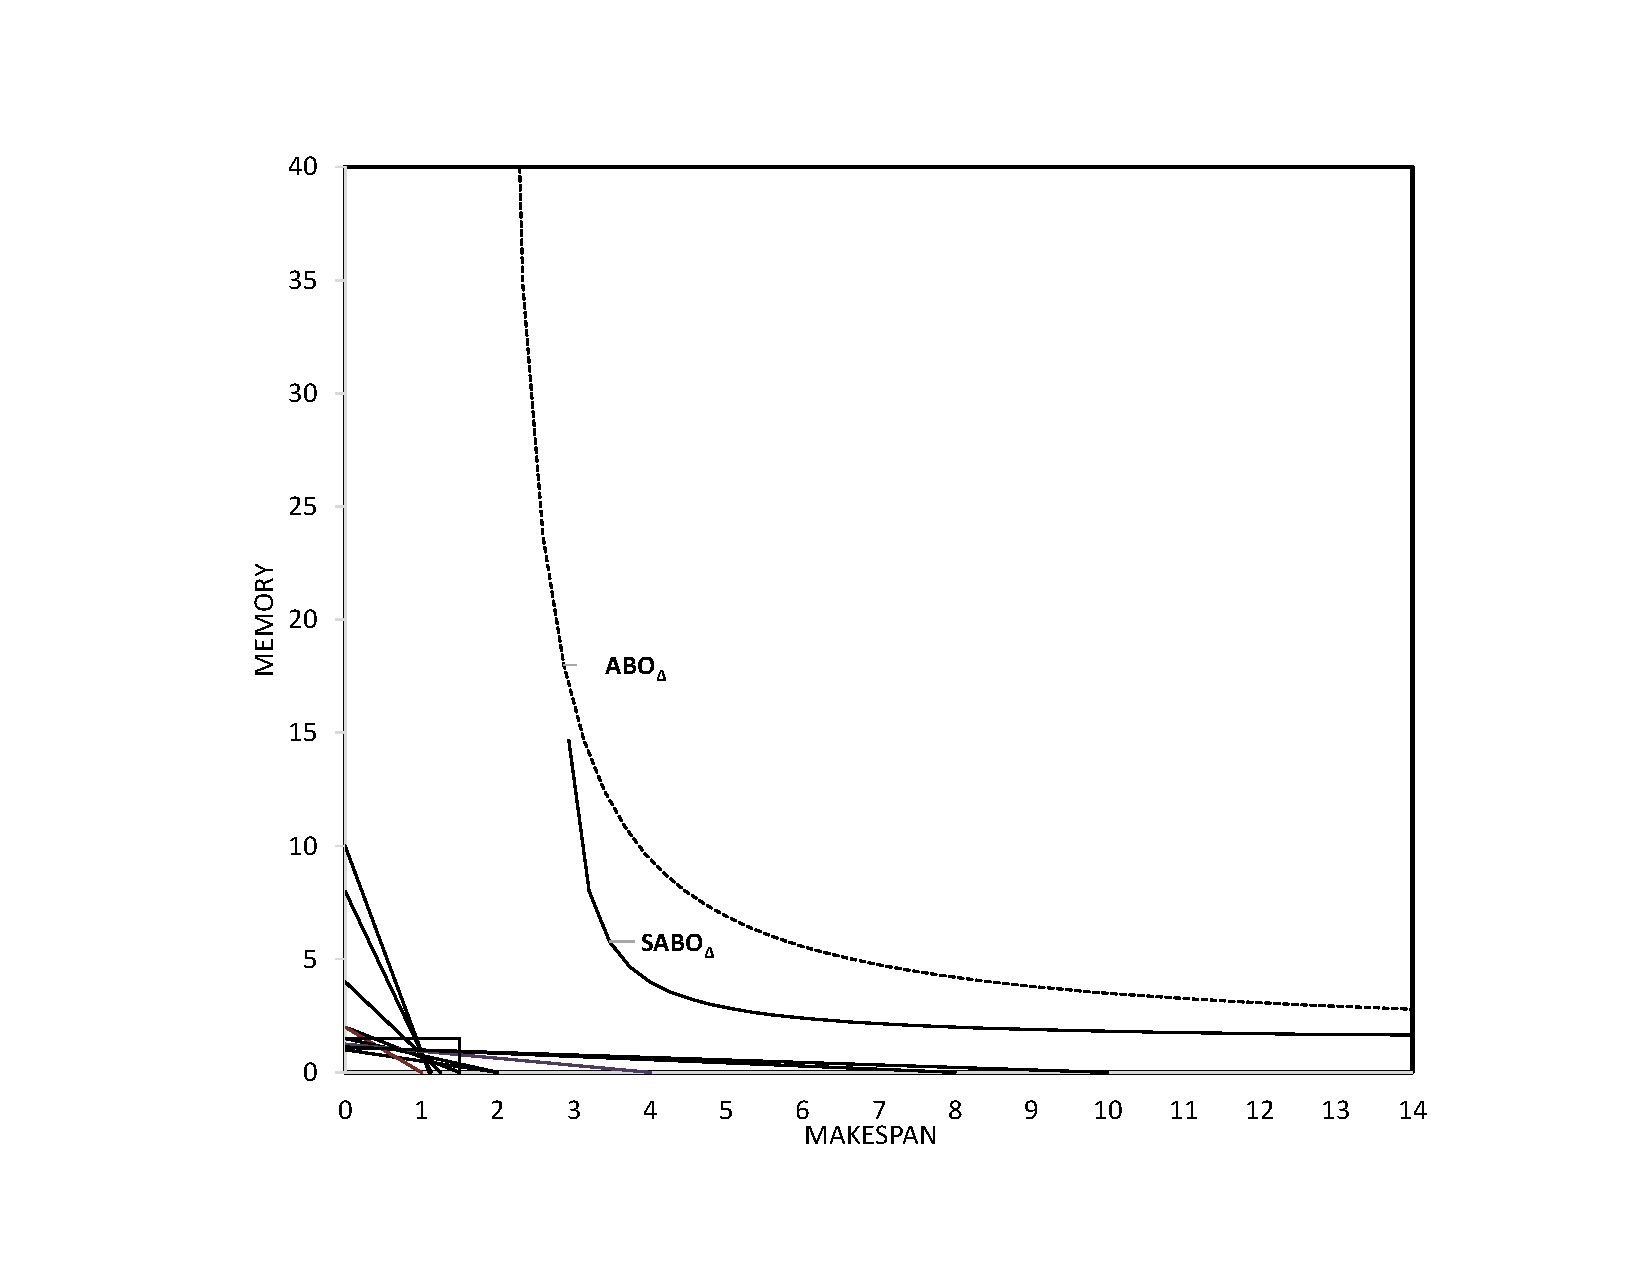
\includegraphics[width=\textwidth]{m5alpha2rho133.pdf}
           \caption{$m=5$, $\alpha^2=2$, $\rho_1=\rho_2=4/3$}
           \label{fig:ch5-3.1}
         \end {subfigure} %
         
         \begin{subfigure}[b]{0.5\textwidth}
           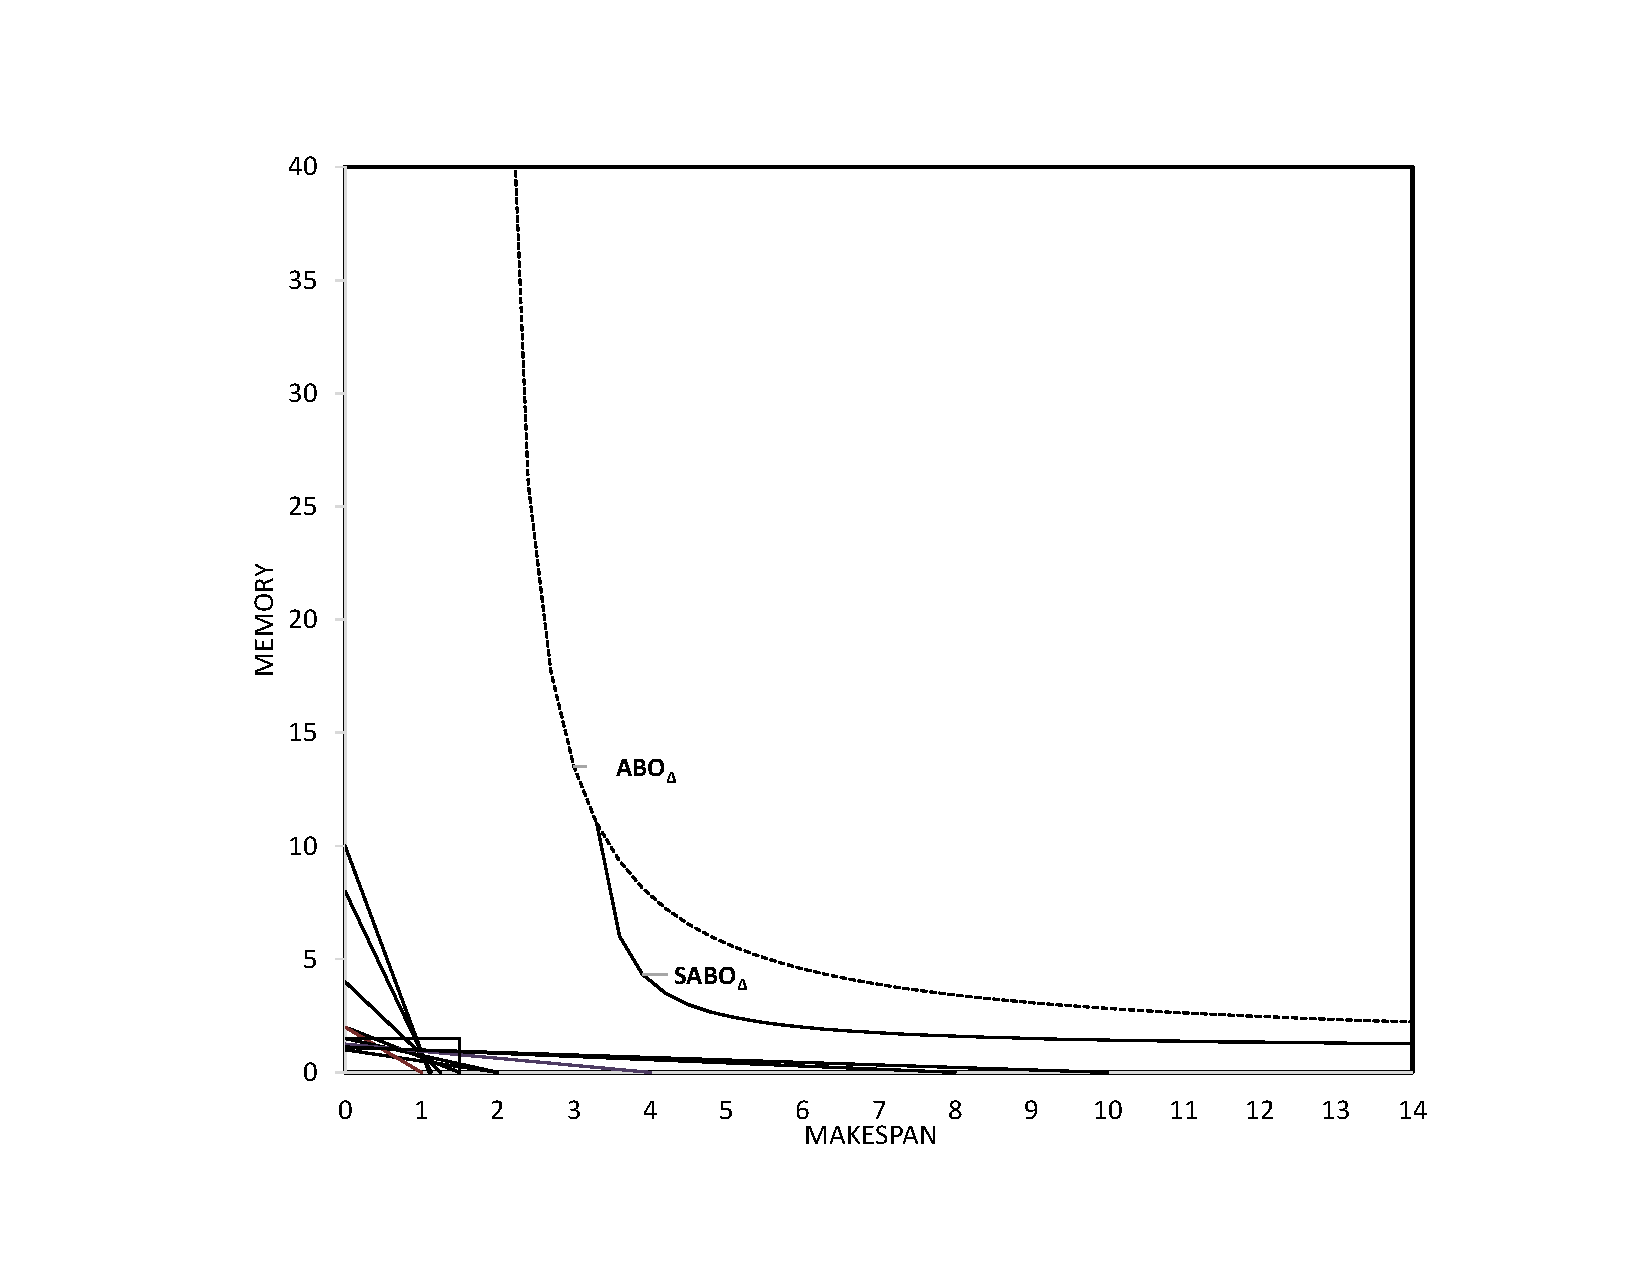
\includegraphics[width=\textwidth]{m5alpha3rho1.pdf}
           \caption{$m=5$, $\alpha^2=3$, $\rho_1=\rho_2=1$}
           \label{fig:ch5-3.2}
         \end {subfigure} %
         
         \begin{subfigure}[b]{0.5\textwidth}
           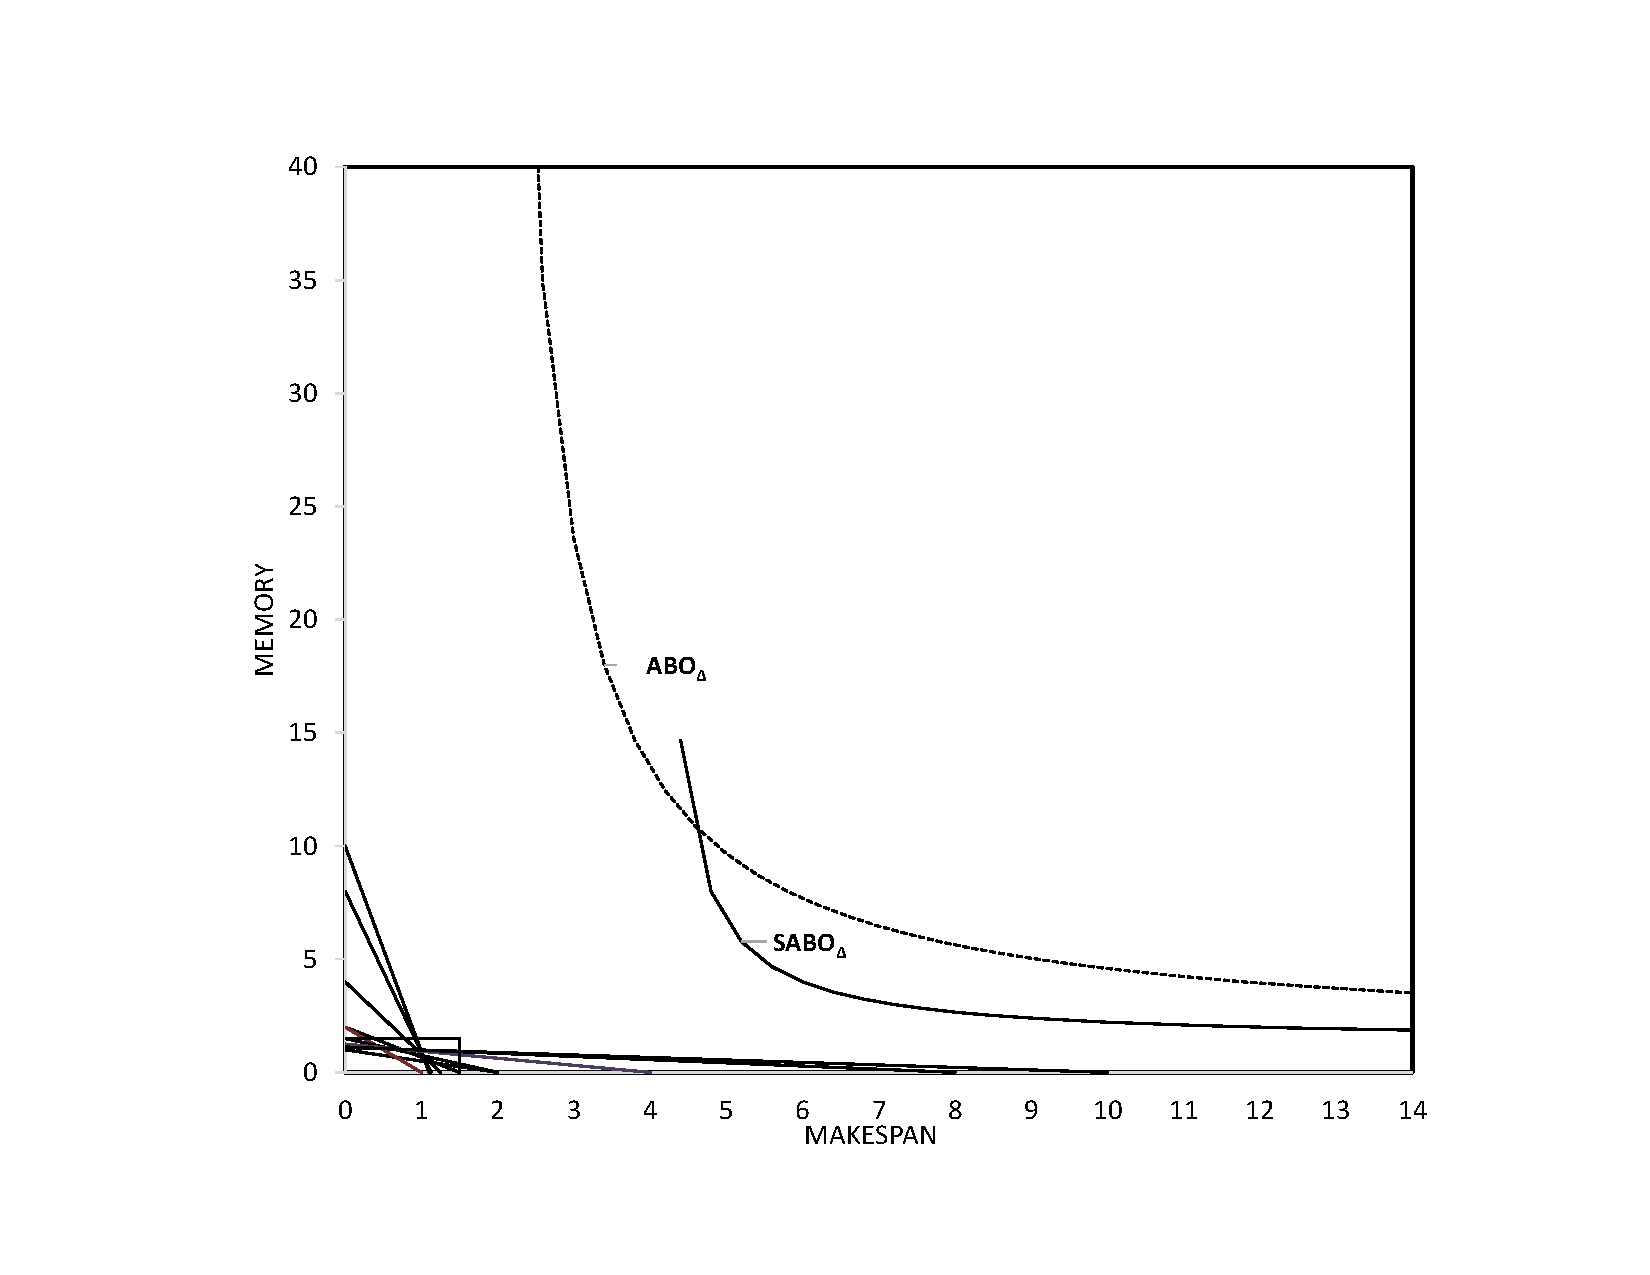
\includegraphics[width=\textwidth]{m5alpha3rho133.pdf}
           \caption{$m=5$, $\alpha^2=3$, $\rho_1=\rho_2=4/3$}
           \label{fig:ch5-3.3}
         \end{subfigure} %
       
         \caption{Memory-Makespan graph for $SABO_\triangle$ and $ABO_\triangle$. The bold lines represent impossibilities in tradeoff between guarantees.}
         \label{fig:ch5-3}
       \end{figure*}
       
    To better understand the tradeoff between memory consumption and makespan Figure~\ref{fig:ch5-3} shows memory-makespan guarantees for the two algorithms.  The bold lines shows impossibilities in the tradeoff between makespan and memory and means that no algorithm can guarantee better tradeoff than this. \cite{10.1109/IPDPS.2008.4536292} discusses about these impossibilities in context of $SBO_\triangle$ algorithm.
   
   The graph shows that for higher values for $\alpha$ the  algorithm $ABO_\triangle$ have better tradeoff between memory-makespan than that of  $SABO_\triangle$. For $\alpha\rho_1\geq 2$,  $ABO_\triangle$ always have better guarantee on makespan than $SABO_\triangle$. So, a schedule more centric to optimize makespan should follow $ABO_\triangle$ algorithm. And a memory centric schedule should follow $SABO_\triangle$ as the algorithm always has better guarantee on memory. 
   
   As a system designer, one always want to pick the algorithm and parameters that is best tradeoff between makespan and memory consumption.  Depending on the guarantee, one should either pick $ABO_\triangle$ or  $SABO_\triangle$  for scheduling tasks.  For instance, if you want to guarantee a makespan  less than 3 as in the case depicted in Figure~\ref{fig:ch5-3.2}, you should use  $ABO_\triangle$. However if you  want a better guarantee on memory, you should always use  $SABO_\triangle$ for task scheduling.
     
                 
    \bodychapter{CONCLUSION AND FUTURE WORK}\label{ch6}
            
    This thesis studies the effect on uncertainty in the processing time of tasks on scheduling for parallel and distributed machines. In particular, it investigates how allowing tasks to execute on different machines can help dealing with not knowing the processing time of tasks accurately. The thesis proposes three replication strategies, provides approximation algorithm in each case and a lower bound on the best achievable approximation in one of the case. Further to limit memory consumption the thesis presents two memory-aware bi-objective algorithms, one of which chooses only critical tasks to replicate and limits memory consumption.
    
    The various strategies allow to trade the number of replication for a better guarantee. The results of these strategies show that a better guarantee can be achieved with fewer replication than that can be achieved by putting the data of a task on only one machine and even a small amount of replications can improve the guarantee significantly. These observations concludes that deploying the data on multiple machines can be an effective way of dealing with processing time uncertainties.
    
    The bi-objective algorithms proposed in this thesis, schedule the memory intensive tasks and the processing time intensive tasks differently and optimizes both the objectives. One of the algorithms, chooses processing time intensive tasks to replicate and achieves better guarantee for higher values of $\alpha$.
    
    There are some open problems which can be explored further. Better lower bounds might help understanding the problem better: clearly when $\alpha$ is low, the problem is no different than the offline problem,and when it is large, the problem converges to the non-clairvoyant online problem. Having a clearer idea of where the boundary is will certainly prove useful in understanding how much can be gained using data replication. Also, while replicating data using groups of processor proved effective, more general replication policies can certainly lead to better guarantees.
    
    
    
   
    
    

    
                  
                  
                                     
    
   



\startbib

 \bibliography{final}

\finishbib

\end{document}